%\documentclass[twoside]{report}
\documentclass[10pt, twoside]{report}

%%%%% ADDED TO SUPPORT TT BOLD FACES %%%%
\DeclareFontShape{OT1}{cmtt}{bx}{n}{<5><6><7><8><9><10><10.95><12><14.4><17.28><20.74><24.88>cmttb10}{}
\renewcommand{\ttdefault}{pcr}
%%%%% END %%%%%%%%%%%%%%%%%%%%%%%%%%%%%%% 
\usepackage{atbegshi,picture}
\AtBeginShipout{\AtBeginShipoutUpperLeft{%
  \put(\dimexpr\paperwidth-1cm\relax,-1.5cm){\makebox[0pt][r]{
\includegraphics[width=3cm]{figs/inno.png}}}%
}}

\usepackage[utf8]{inputenc}
\usepackage[T2A]{fontenc}
\usepackage[russian, english]{babel}
\usepackage{blindtext}

\newenvironment{bottompar}{\par\vspace*{\fill}}{\clearpage}

\usepackage{cite}
\usepackage{amsmath,amsfonts}

\usepackage{amsthm}
\newtheorem{theorem}{Theorem}
\newtheorem{corollary}{Corollary}
\newtheorem{lemma}{Lemma}
\newtheorem{proposition}{Proposition}
\theoremstyle{definition}
\newtheorem{definition}{Definition}
\theoremstyle{remark}
\newtheorem*{remark}{Remark}
\theoremstyle{remark}
\newtheorem*{example}{Example}


\usepackage{pdfpages}
\usepackage{float}
\usepackage{graphicx}
\usepackage{array}
\usepackage{multirow,array}
\usepackage{caption}
\usepackage{subcaption}
\usepackage{hyperref}
\usepackage{paralist}
\usepackage{listings}
\usepackage{zed-csp}
\usepackage{fancyheadings}
\usepackage{color}

\definecolor{mygreen}{rgb}{0,0.6,0}
\definecolor{mygray}{rgb}{0.5,0.5,0.5}
\definecolor{mymauve}{rgb}{0.58,0,0.82}
\definecolor{orange}{rgb}{1.0,0.64,0}

\usepackage{upgreek} 
\usepackage{bm}
\usepackage{hyperref}
\usepackage{setspace}
\usepackage{booktabs}
\usepackage{multirow}
\usepackage{longtable}
\usepackage[font=singlespacing, labelfont=bf]{caption}


\usepackage{enumitem}
\newlist{inlinelist}{enumerate*}{1}
\setlist*[inlinelist,1]{%
  label=(\arabic*),
}

\usepackage{listings}


\pagestyle{fancyplain}

% remember section title
\renewcommand{\chaptermark}[1]%
	{\markboth{\chaptername~\thechapter~--~#1}{}}

% subsection number and title
\renewcommand{\sectionmark}[1]%
	{\markright{\thesection\ #1}}

\rhead[\fancyplain{}{\bf\leftmark}]%
      {\fancyplain{}{\bf\thepage}}
\lhead[\fancyplain{}{\bf\thepage}]%
      {\fancyplain{}{\bf\rightmark}}
\cfoot{} %bfseries


\newcommand{\dedication}[1]
   {\thispagestyle{empty}
     
   \begin{flushleft}\raggedleft #1\end{flushleft}
}

\graphicspath{ {figs/} }

\usepackage{xcolor}

\colorlet{punct}{red!60!black}
\definecolor{delim}{RGB}{20,105,176}
\colorlet{numb}{magenta!60!black}

\lstdefinelanguage{json}{
    basicstyle=\normalfont\ttfamily,
    numbers=left,
    numberstyle=\scriptsize,
    stepnumber=1,
    numbersep=8pt,
    showstringspaces=false,
    breaklines=true,
    frame=lines,
    literate=
     *{0}{{{\color{numb}0}}}{1}
      {1}{{{\color{numb}1}}}{1}
      {2}{{{\color{numb}2}}}{1}
      {3}{{{\color{numb}3}}}{1}
      {4}{{{\color{numb}4}}}{1}
      {5}{{{\color{numb}5}}}{1}
      {6}{{{\color{numb}6}}}{1}
      {7}{{{\color{numb}7}}}{1}
      {8}{{{\color{numb}8}}}{1}
      {9}{{{\color{numb}9}}}{1}
      {:}{{{\color{punct}{:}}}}{1}
      {,}{{{\color{punct}{,}}}}{1}
      {\{}{{{\color{delim}{\{}}}}{1}
      {\}}{{{\color{delim}{\}}}}}{1}
      {[}{{{\color{delim}{[}}}}{1}
      {]}{{{\color{delim}{]}}}}{1},
}

\begin{document}\sloppy
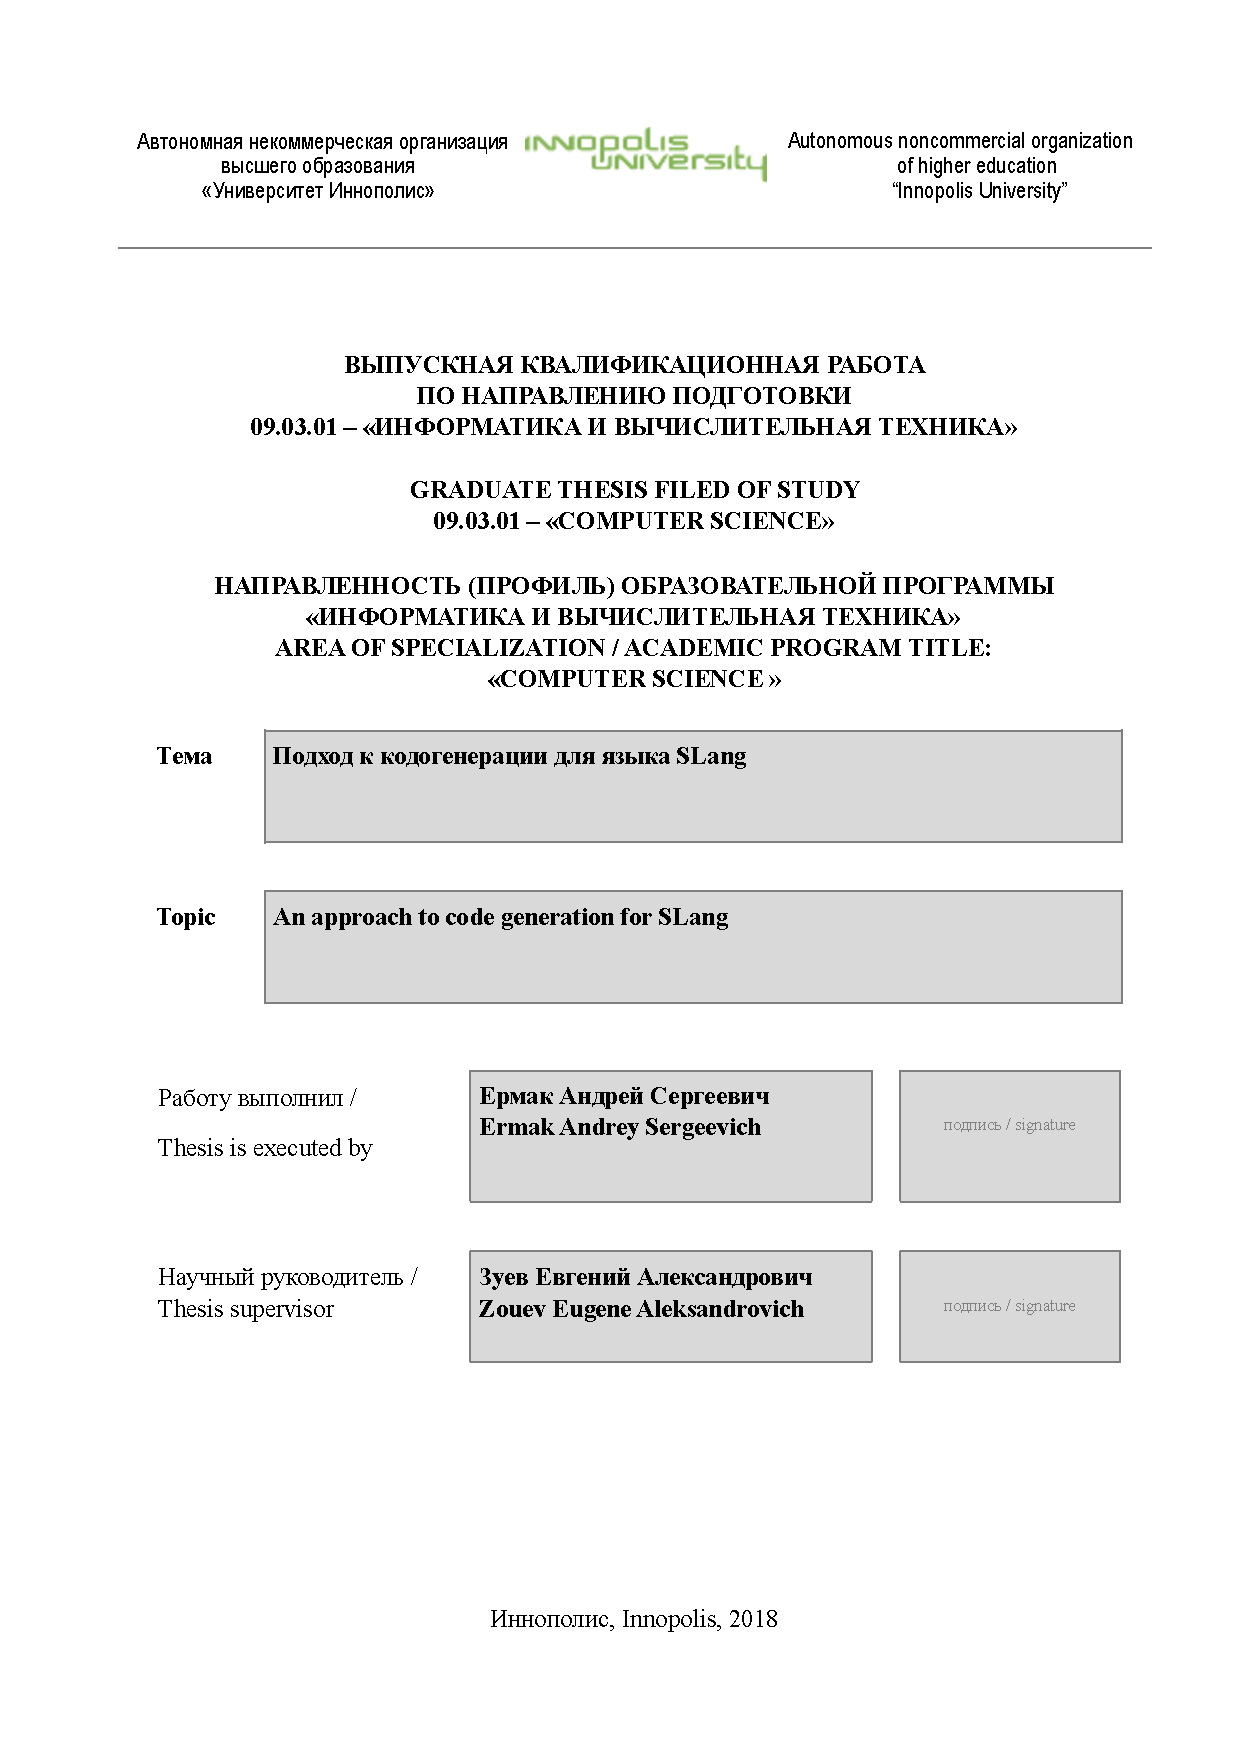
\includepdf[pages=-]{chapters/BST.pdf}
% \begin{titlepage}

\begin{center}

\textbf{\Large{An approach to code generation for SLang}}
\vspace{4cm}

\textbf{\Large Innopolis University} \\

\vspace{0.60cm}

{\Large Thesis submitted to The Innopolis University in conformity with the
requirements for the degree of Bachelor of Science.}

\vspace{6cm}

{\Large presented by}

\vspace{0.40cm}

\textbf{\Large Andrey Ermak}
\vspace{0.40cm}

{\Large supervised by}\\
\vspace{0.40cm}
{\bf\Large Eugene Zouev}\\
\vspace{0.60cm}
%{\Large Date}



\end{center}
\end{titlepage}



\tableofcontents
% \listoftables
% \listoffigures

\begin{abstract}
In this thesis work, an approach to code generation for brand new programming language is considered. 
% Целевой платформой для кодогенерации был выбран язык Си из-за его распространённости под большинство архитектур. 
The C language was chosen as the target platform for code generation because of its prevalence for most architectures.

% В процессе работы был реализован транслятор из AST языка SLang в код языка Си. Для чего был придуман и реализован подход трансляции, базирующийся на использовании шаблонов целевого языка.
During the work, the translator from AST of SLang language to C code was implemented. For this task, the translation approach based on the using of target language templates was invented and implemented.
\end{abstract}
\setcounter{page}{2}

%!TEX root = root.tex

\chapter{Introduction}
\label{chap:intro}
\chaptermark{Optional running chapter heading}

\section{Motivation}
The SLang now is in development, and there is an issue of compiler implementing. It is a critical step in language creation because the implementation of the compiler will influence its distribution and efficiency.

There are several ways to solve this issue: 
\begin{itemize}
    \item The first is just to implement compiler directly. Obviously, it is the most complicated way, because of plenty specifics in implementation depending on hardware, which imposes many issues;
    \item The second one is to implement frontend in one of the compilers like GCC or LLVM. It is a good solution, but the backends of these compilers are implemented not for all hardware architecture, like Elbrus architecture which does not support LLVM;
    \item The third way is to implement frontend of one of the virtual machines like .NET or JVM, it is a good and easy way, but there are issues too, e.g., the JVM does not support multiple inheritance, which is supported in SLang, or, VM are slowly in general;
    \item And the last is to implement source-to-source translation in one of the popular programming languages like C. The main advantages of this approach is widely supporting of C languages by the most of hardware --- from primitive microcontrollers to modern OS. Also, it is more efficient and faster because of compilation;
\end{itemize}
Considering the above, we chose the last one --- Source-to-source interpretation into the C programming language.
\label{sec:section}
\chapter{Literature Review}
\label{chap:lr}
\chaptermark{Literature Review Heading}

The purpose of this thesis is to develop an approach to code generation from SLang programming language to some target platform and to implement it. The C language was chosen as the target platform because of it is wide distribution.

It is, basically, quite a complicated task that is subject to complex and differentiated approaches, consisting of many problems. Some of them include translating basic semantic notions and expressions from Slang to C, as well as object-oriented programming issues that lay quite far from trivial, with C being a procedural, not an object-oriented language. To get more familiar with this area of research, a literature review was performed.

It seems logical to divide this global task into several smaller ones:
\begin{itemize}
\item Code generation issues --- the key part of this thesis and therefore the area that deserves the most attention.
\item Intermediate Representation --- also a part of the thesis, so the approaches to it should be considered as well.
\item Object-Oriented Programming --- quite complicated and interesting task -- to implement OOP paradigm in an imperative-only programming language like C.
\end{itemize}

\section{Code generation issues}

The first thing in desperate need to be discussed is code generation, as it what needs to in the course of the thesis.

In this thesis, code generation is a process of generating source code from the intermediate representation, which means the translation from semantic blocks of one language to another.

The problems of code generation were considered in some papers which are related to source-to-source code generation. For instance, three main techniques applicable for the task are explored in a work by Lossing et al.\cite{Lossing2016}:
\begin{enumerate}
    \item ``To move the declaration at the main scope level.''
    \item ``To mimic a conventional binary compiler and to transform typedef and declaration  statements  into  memory  operations,  which  is,  for  instance, performed in Clang.''
    \item ``To extend def-use chains and data dependence graphs to encompass effects on the environment and the mapping defining named types.''
\end{enumerate}

Besides, authors were devoted to optimization of control flow graphs \cite{wikiCFG} for source-to-source code generation. They justified the choice to make a   source-to-source compiler for C, because of portability and stability of the language that allows for easier maintenance.

Lossing et al. also discuss suitability and problems of Data Dependence Graphs \cite{markheffernankentwilken2005} for source-to-source compilation, as well as suggest several workarounds for problems related to working with memory. however, this approach does not cover all the language use cases,   and because of this, authors suggest a solution called Effects dependence graph, which is ``an extension of the Data Dependence Graph taking into account the environment and the type declaration functions.''

Another approach to the problem is performing code transformation using AST\cite{wikiAST} representation. There is a toolset that implements that approach based on the Xevolver framework. The critical feature of the project is said to be ``code transformations based on the analyzed syntax of the target code, rather than just a text level transformations such as C preprocessor''\cite{Suda2017}.

This tool provides several kinds of abstractions for code transformation framework:
\begin{itemize}
\item ``an abstract view of temporary files.''
\item ``an abstract view of combinations of code transformations.''
\item ``a viewer that incorporates the above two kinds of abstractions.''
\end{itemize}

Based on the facts mentioned above, it is clear that some existing approaches and tools are allowing to solve the task of code generation and specifically source-to-source translation, and are possible to use to implement the proposed system.

\section{Intermediate Representation}
The intermediate representation is a way to represent source code in the form of a data structure or IR code, which keeps the semantics of the program. An IR is allowed to perform code optimization and easier translation for a target platform.

As mentioned above, there are several approaches to representing the source code, and one of them is a   graph-based IR which very closely resembles Control Flow Graph. Click and Paleczny described such kind of implementation in 1995 \cite{Click1995}. Here, the Petri networks are used to make a model. As the result of that work, authors achieve 6.3\% faster compile time using the described approach.

Based on the materials of the paper mentioned above, now it is clear that it is possible to implement intermediate representation with use of the control flow graph.

\section{Object Oriented Programming}

OOP is a widely used paradigm, and SLang also implements it. 
It is an entirely exciting and complicated task to implement it in a procedural language like C.

Here are some materials that describe the approaches how OOP can be implemented in C language. The first one \cite{Ducournau2009} describes several implementation techniques of OOP, such as:

\begin{itemize}
\item Single   Subtyping
\item Subobjects   (SO)
\item Coloring   (MC/AC)
\item Binary   Tree   Dispatch   (BTD)
\item Perfect   Hashing   (PH)
\item Incremental   Coloring   (IC)
\item Accessor   Simulation   (AS)
\item Caching   and   Searching   (CA)
\end{itemize}
Another paper \cite{Trudel2012a} is devoted to description and analysis of several tools for translating C to some OO languages like Eiffel, C\# or Java. The main idea here is to demonstrate advantages of translating C to Eiffel with C2Eiffel tool. Furthermore, internal work of this tool is described, so it seems to be convenient for the thesis topic.

The most exciting part of this section is the ``Object-oriented programming with ANSI-C'' book \cite{Schreiner2011}.
It is like a cookbook of OOP in C, which describes the process of implementing OOP in C very clearly and in details.
There are many references to this book in scientific papers and on the internet.

Using materials of this book, it is possible to dig deep into details and nuances of object-oriented programming in C.

\section{Conclusion and next steps}

In the course of performing this literature overview, the key concepts related to this thesis were considered, the vision of situation was formed, and the next steps are suggested:
\begin{enumerate}
    \item Create the design of IR
    \item Write AST-parser to IR
    \item Write module that converts IR to target programming language
    \item Implement the OOP part
\end{enumerate}

\chapter{The proposed architecture}
\label{chap:met}
\lstdefinestyle{customc}{
    belowcaptionskip=1\baselineskip,
    breaklines=true,
    frame=L,
    xleftmargin=\parindent,
    language=C,
    showstringspaces=false,
    basicstyle=\footnotesize\ttfamily,
    keywordstyle=\bfseries\color{mymauve},
    commentstyle=\itshape\color{mygreen},
    identifierstyle=\color{blue},
    stringstyle=\color{orange},
    numbers=left,
    captionpos=b
}
  
\lstset{escapechar=@,style=customc}

Authors of the language propose the following pipeline of the compilation of software written in SLang (Figure \ref{fig:compiler_pipeline}). The compiler starts with a parser which parses the source code in SLang into an AST, for it to be then converted into a kind of intermediate representation, which is further converted to a target platform code.

\begin{figure}[h!]
    \centering
    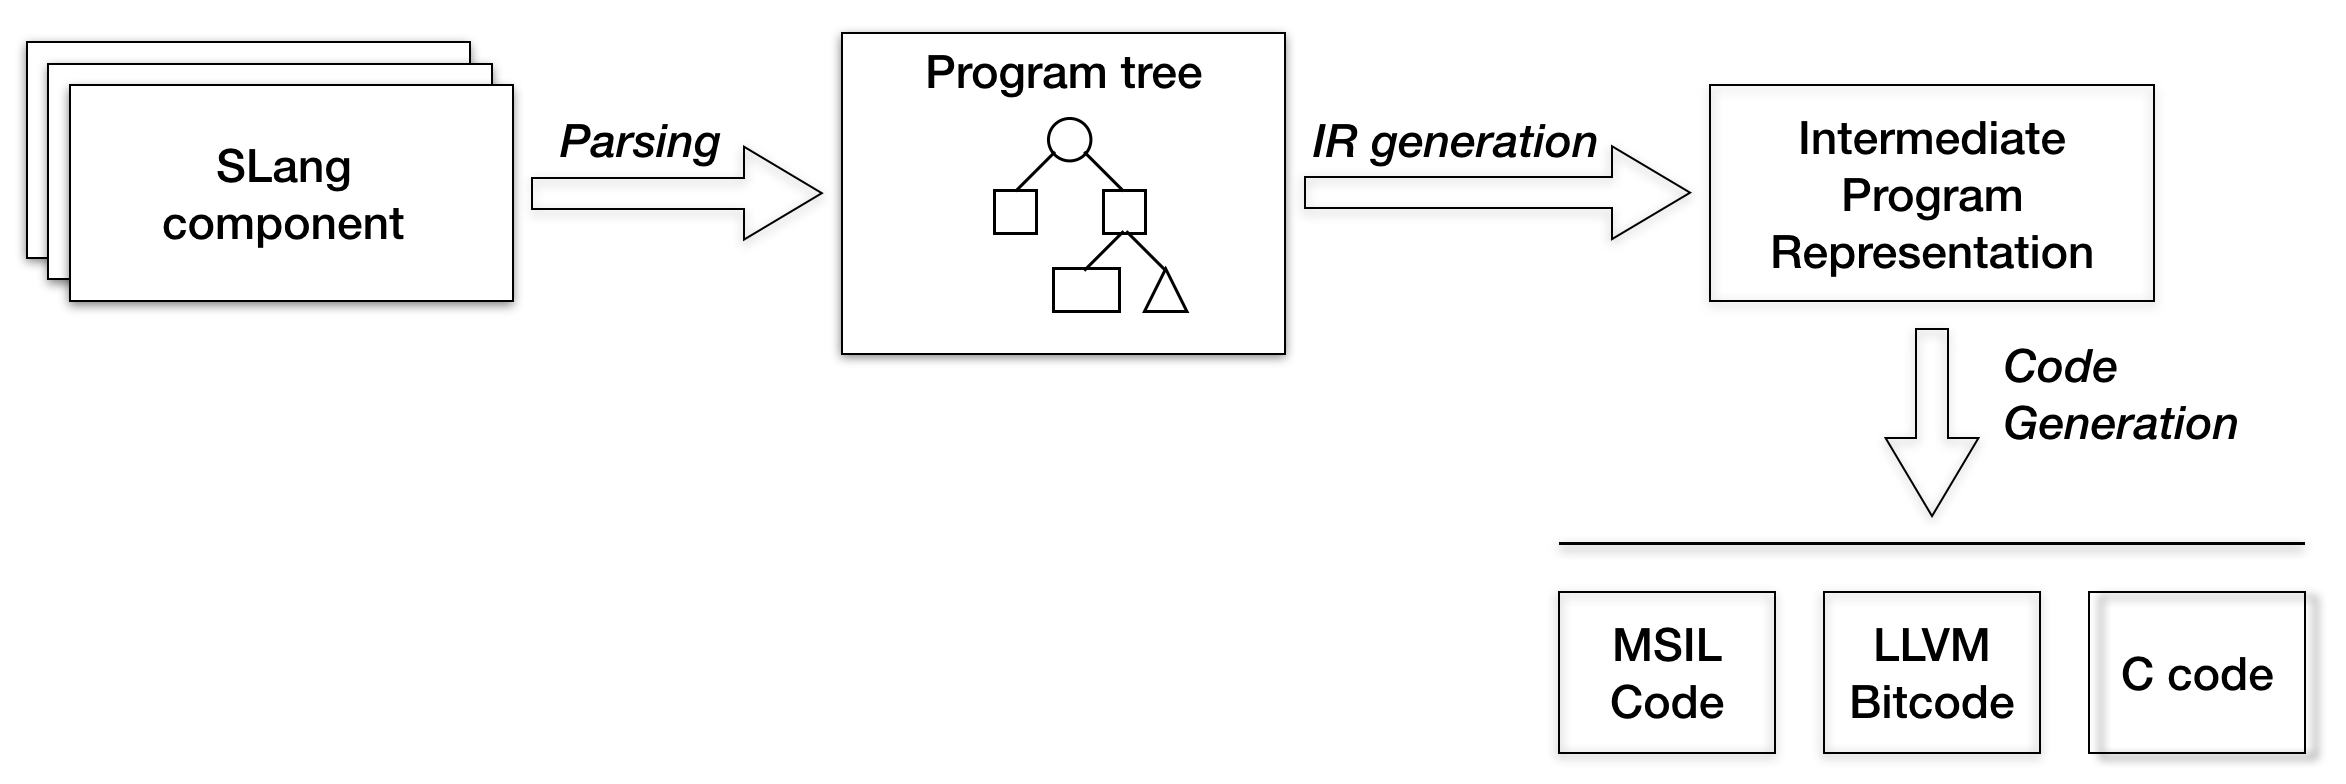
\includegraphics[width=\linewidth]{compiler_pipeline.png}
    \caption{Compiler pipeline}
    \label{fig:compiler_pipeline}
\end{figure}

As a part of a process of the compiler development, three kinds of platforms are proposed to perform code generation into, namely .NET, LLVM and C language. In this work, implementation of code generation in C is developed. This decision is motivated by the fact that multiple architectures existing nowadays have a C compiler written for them, which includes proprietary like Elbrus \cite{Elbrus} or for embedded systems which only have a C or assembler compiler.

\section{Compiler frontend, middle-end and backend}
The notion of a modern compiler implies modularity, or division into modules, which include frontend, backend and sometimes middle-end. This way of structuring allows dividing compiler development into language syntax description, code generation for specific hardware and optimization respectively, which, in its turn, proved to help to simplify both the process of compiler development and the process of it being expanded by third-party developers.

With modular compiler architecture, a developer of a new language needs to describe the syntax and rules of translation of language constructs into some high-level representation constructs, instead of caring about how these constructs are implemented on the low level in any particular architecture.

In other words, modularity allows developers to reuse already existing components to expand language-platform variety, which led to compilers designed this way being called retargetable.

On the picture described above (Fig \ref{fig:compiler_pipeline}), the front-end is the parser, the middle-end consists of IR generation and code generation, and backend is necessarily the target platform, for which code generation is performed.

As we need to find out how to make a system that works, it is necessary to review existing works in the field. In this section, we will mostly concentrate on two most popular open source compilers, namely GCC and LLVM, due to them being actively developed by open source community and incredibly widely used, which implies they are reliable enough to be exemplary.
 

\subsection{Compiler frontend}
The compiler frontend is a part of a compiler translating source code to some intermediate representation. 
Usually, frontend pipeline includes some or all of the following steps in the specified order:
\begin{enumerate}
    \item \textbf{Lexical analysis}
    \begin{itemize}
        \item \textbf{Line reconsruction} changes strings of literals into a parser-suitable format, usually deleting comments, tabulations, unnecessary spacing and new line characters;
        \item \textbf{Preprocessing} applies macros or others built-in language preprocessing functions; 
        \item \textbf{Tokenization} breaks the preprocessed code into lexical tokens, which can be interpreted by compiler to construct IR;
    \end{itemize}
    \item \textbf{Syntax analysis} parses the set of tokens into an \textit{abstract syntax tree (AST)} or other type of IR;
    \item \textbf{Semantic analysis} adds metainformation to IR tokens, such as type or access modifiers, and performs error checking; 
\end{enumerate}

GCC, for instance, provides frontends for C, C++, Objective-C, Fortran, Ada, and Go languages \cite{GNU}, while LLVM can use frontends based on the GCC 4.2 parsers as well as its frontends \cite{LLVM_features}.

\subsection{Compiler middle end (ordinary optimizer)}

This step performs optimizations on the IR level. The advantage of it is that powerful optimizers do not usually allocate memory until optimization is performed, and only do it when it is clear that individual variables do not exist outside registers, so they do not need memory allocation. Moreover, it makes possible to determine the order in which variables are to be allocated in memory so that maximal amount of them is cached, which, in its turn, positively affects performance.

\subsubsection{GCC}
GCC middle-end is explicitly defined and performs SSA-based\footnote{\textbf{Static Single Assignment form (SSA)} is a property of an IR, which requires that each variable is assigned exactly once, and every variable is defined before it is used. \cite{SSA_wiki} } optimizations of a program translated to GIMPLE (one of a few intermediate representations in GCC), and then translates GIMPLE into RTL\footnote{\textbf{Register Transfer Language (RTL)} is a kind of intermediate representation (IR) that is very close to the assembly language, such as that which is used in a compiler. \cite{RTL_wiki}}, where more low-level optimizations are performed, and then, after it is done, the optimized program in RTL is redirected to compiler back-end.

\subsubsection{LLVM}
In LLVM, middle-end is explicitly defined as well and is utilized to translate the program into an intermediate language called bit code language, perform SSA optimizations in bit code, and redirect the program to back-end afterward.

\subsubsection{SLang}
This step will perform optimizations and construct data structures for the C language, as C, for example, does not have classes as language constructs, which implies the need to represent them as sets of structures and functions related to them.

\subsection{Compiler backend}
The backend is a part of a compiler which generates code and performs optimizations for a specific CPU architecture.

\begin{itemize}
    \item \textbf{LLVM} supports multiple architectures, including X86, X86-64, and ARM. The full list is available on the LLVM website \cite{LLVM_features};
    \item \textbf{GCC} is older than LLVM and supports more architectures. The list of all supported architectures is presented on the GCC website \cite{GCCback};
\end{itemize}


\section{Abstract Syntax Tree (AST)}
AST is a way to represent a program in a tree form. Each node of AST denotes a construct occurring in the source code, written in a programming language. The tree is called abstract since not all syntactic details are preserved. Because of that, programs written in different programming languages but doing the same thing may well have the same AST structure.

Since one of the objectives of this thesis is the design of AST representation, let us now look at what options exist presently.

\subsection{Variants of representation}

Consider AST for GCC and LLVM:
\begin{itemize}
    \item \textbf{GCC} allows us to get plenty of variants of program representation. Using the command ``gcc-7 test.c -fdump-tree-all'', it is possible to generate many files that appear in the course of performing optimizations. One of them is a ``.gimple'' file that contains the code of a program in GIMPLE language, Listing \ref{lst:GCC_gimple}. In an ``.optimized'' file, Listing \ref{lst:GCC_gimple_optimized}, there is an optimized version of the code in GIMPLE.

    \item In \textbf{LLVM}, CLang is a part of LLVM toolchain, or, to be more specific, the compiler frontend for C, C++ and Objective-C programming languages \cite{CLangDoc}. 
    CLang contains a part responsible for AST construction, which uses the kind of AST that slightly differs from those used in other compilers, for it to resemble C++ code structure, for instance, ``parenthesis expressions and compile-time constants are available in an unreduced form in the AST'' \cite{CLangAST}.
    This feature makes CLang AST more suitable for refactoring tools.
\end{itemize}

Consider the following program in C:
\begin{lstlisting}[caption={Example of a C source code}, label=lst:C_Example]
    // test.c
    int main() {
        int a = 1; 
        int b = 2;
        return a + b;
    }
\end{lstlisting}

Obviously, this program can be optimized into call of \textit{return 3;} in the \textit{main} function. Let us now consider the ways of this program being optimized by two compilers mentioned above.


In Clang, we can output the AST representation of a program to the terminal. For the previous example, the tree looks as follows:

\begin{lstlisting}[morekeywords={FunctionDecl, CompoundStmt, DeclStmt, VarDecl, IntegerLiteral, ReturnStmt, TranslationUnitDecl, ImplicitCastExpr, DeclRefExpr}, caption={CLang AST}, label=lst:CLang_AST]
    $ clang -Xclang -ast-dump -fsyntax-only test.c

    TranslationUnitDecl 0x5aea0d0 <<invalid sloc>>
    ... cutting out internal declarations of clang ...
    `-FunctionDecl 0x7ff950058400 <test.c:1:1, line:6:1> line:1:5 main 'int ()'
    `-CompoundStmt 0x7ff950058740 <col:11, line:6:1>
      |-DeclStmt 0x7ff950058570 <line:2:1, col:10>
      | `-VarDecl 0x7ff9500584f0 <col:1, col:9> col:5 a 'int' cinit
      |   `-IntegerLiteral 0x7ff950058550 <col:9> 'int' 1
      |-DeclStmt 0x7ff950058620 <line:3:1, col:10>
      | `-VarDecl 0x7ff9500585a0 <col:1, col:9> col:5 b 'int' cinit
      |   `-IntegerLiteral 0x7ff950058600 <col:9> 'int' 2
      |-DeclStmt 0x7ff9500586d0 <line:4:1, col:10>
      | `-VarDecl 0x7ff950058650 <col:1, col:9> col:5 used c 'int' cinit
      |   `-IntegerLiteral 0x7ff9500586b0 <col:9> 'int' 3
      `-ReturnStmt 0x7ff950058728 <line:5:1, col:8>
        `-ImplicitCastExpr 0x7ff950058710 <col:8> 'int' <LValueToRValue>
          `-DeclRefExpr 0x7ff9500586e8 <col:8> 'int' lvalue Var 0x7ff950058650 'c' 'int'
\end{lstlisting}


% \begin{lstlisting}[frame=L, numbers=left, language=C, basicstyle=\footnotesize, caption=GCC AST\label{lst:GCC_AST}]
% gcc tree
% \end{lstlisting}
% [discription]

Both compilers allow us to have a look at IR and observe opimizations being done. Here is how the bitcode looks fot the AST above:
%Оба компилятора позволяют рассмотреть IR и понаблюдать за проходками оптимизации этой программы:

\begin{lstlisting}[escapeinside={\%*}{*)}, caption={LLVM bitcode in SSA form}, label={lst:LLVM_bitcode}]
    $ clang -c -emit-llvm test.c -o test.bc
    $ llvm-dis test.bc -o test.ll // SSA
    $ clang -S -emit-llvm test.c -o test.ll

    ; ModuleID = 'test.c'
    define i32 @main() #0 {
        %1 = alloca i32, align 4
        %2 = alloca i32, align 4
        %3 = alloca i32, align 4
        store i32 0, i32* %1, align 4
        store i32 1, i32* %2, align 4
        store i32 2, i32* %3, align 4
        %4 = load i32, i32* %2, align 4
        %5 = load i32, i32* %3, align 4
        %6 = add nsw i32 %4, %5
        ret i32 %6
      }
\end{lstlisting}

The bitcode in the listing above is generated in SSA form. The @ prefix denotes global identifiers like function names, the \# symbol serves as a prefix for a code block ID, and the \% symbol denotes local identifiers like variable declarations. In this listing, memory allocation blocks are explicitly observable, as well as assignments and loading of assigned values to further use them to compute and return the result.

The GIMPLE code is more similar to C, compared to bitcode. For instance, in the listing \ref{lst:GCC_gimple} it is possible to find variable definition and declaration that looks just like in C.

\begin{lstlisting}[frame=L, language=C, numbers=left,basicstyle=\footnotesize, caption={GCC gimple in SSA form}, label={lst:GCC_gimple}]
    $ gcc-7 test.c -fdump-tree-all
    $ cat test.c.049t.ssa

    ;; Function main (main, funcdef_no=0, decl_uid=1809, cgraph_uid=0, symbol_order=0)
    
    main ()
    {
      int b;
      int a;
      int D.1814;
      int _3;
    
      <bb 2> [0.00%]:
      a_1 = 1;
      b_2 = 2;
      _3 = a_1 + b_2;
    
    <L0> [0.00%]:
      return _3;
    }
\end{lstlisting}

Next, optimized bitcode:
%Далее, оптимизированный код в биткоде:
\begin{lstlisting}[escapeinside={\%*}{*)}, caption=LLVM bitcode optimized, label={lst:LLVM_bitcode_o}]
    $ clang -c -emit-llvm test.c -o test.bc -O1
    $ llvm-dis test.bc -o test.ll

    ; ModuleID = 'test.c'
    define i32 @main() local_unnamed_addr #0 {
        ret i32 3
      }
\end{lstlisting} 
By default, when trying to observe bitcode, one is getting it without optimization. If one wishes to see the optimized code, they will need to compile it with the -O1 flag. In the listing, it is easy to see that the program was minimized as much as possible, and all expressions that did not bring anything useful were cut out. Furthermore, there is one more optimization on the main function, namely the expression ``local\_unnamed\_addr'' being added before the function, which is described in the documentation as follows: ``If the ``local\_unnamed\_addr'' attribute is given, the address is known to not be significant within the module.'' \cite{LLVM_manual}


\begin{lstlisting}[frame=L, language=C, numbers=left,basicstyle=\footnotesize, caption={Release GCC gimple in SSA form}, label={lst:GCC_gimple_optimized}]
    $ gcc-7 test.c -fdump-tree-all -O1
    $ cat test.c.049t.release_ssa

    ;; Function main (main, funcdef_no=0, decl_uid=1809, cgraph_uid=0, symbol_order=0) (executed once)
    
    Released 3 names, 150.00%, removed 3 holes
    main ()
    {
      <bb 2> [100.00%]:
      return 3;
    }
\end{lstlisting}
As we can see, this example also shows full optimization. Moreover, it is worth noting that in GCC, three optimization flags -- -O1, -O2, and -O3 -- are available, to allow for different levels of optimization. In fact, there are many more optimization flags which all have the different meaning, described on the GCC website \cite{GCC_optimizations}.

\section{Intermediate representation}
The intermediate representation is closely connected to AST -- as it is also a way of program representation. Often, AST itself is a form of IR, and other compilers\cite{Non_AST_compilers} can even transform code into non-AST IR omitting the AST stage. 

\subsection{Expressions of IR}
\begin{itemize}
    \item \textbf{LLVM bitcode} mentioned above in examples \ref{lst:LLVM_bitcode} and \ref{lst:LLVM_bitcode_o}. It is a low-level language, similar to assembly language, but unlike assembler, bitcode is not platform-dependent, even though it allows for platform-specific low-level operations.

    \item \textbf{CIL}. Common Intermediate Language designed by Microsoft, and it is a part of the .NET framework. Also similar to assembly language, and is used to represent a program inside the .NET virtual machine.

    \item \textbf{GIMPLE} is GCC intermediate language, as mentioned above. It comes in two flavors: High-Level GIMPLE is a common IR for all GCC front-ends and is generated in the middle end, listing \ref{lst:GCC_gimple}, while Low-Level GIMPLE is generated from the High-Level GIMPLE with the help of control flow graph generated for this purpose. The program in Low-Level GIMPLE is then SSA-optimized, and after that, translated to RTL, which has Lisp-like syntax.

    \item \textbf{C programming language}. For Eiffel, Sather, Esterel, Haskell \cite{GlasgowHaskellCompiler}, Cython. C was chosen to be used as one of the intermediate languages for SLang.
\end{itemize}

\subsection{Advantages}
\begin{itemize}
    \item IR allows compilers to perform multiple passes of program optimization;
    \item IR is some abstraction; therefore it can be used for other languages and other compilers;
    \item IR allows as well as AST perform CPU independent optimizations;
\end{itemize}

% \subsection{Disadvantages}
% \begin{itemize}
%     \item It slows down compilation process;
%     \item In any case, IR imposes restrictions on the language frontend;
%     [EXAMPLE]
% \end{itemize}

\subsection{Auxiliary representations}
There is a number of auxiliary representations commonly used in compilers\cite{UMDIR}:
\begin{itemize}
    \item Abstract syntax tree (AST) --- representation of a program in a tree form;
    \item Control flow graph (CFG) --- a way of representing a program with a graph that describes all possible paths of program execution;
    \item Three-address code (TAC) --- is a most useful way for a compiler to optimize a program. Every instruction in TAC consists of three operands  -- this is the reason why TAC is called this way; %which three operands?
    \item Stack-based representation (SBR) --- is a lower level representation of TAC -- each command of TAC can be converted to a few commands of SBR. SBR has quite a simple syntax, but it is not human-readable; 
\end{itemize}

% \subsection{Restrictions}

\section{Concept}
In this research, the middle-level representation (MLR) of SLang is going to be considered.

MLR is a vital part of a translator, which translates language SLang constructs to corresponding C entities, without loss of functionality. 
As the result of research, the high-level architecture of MLR now consists of the following parts:

\begin{itemize}
    \item \textbf{IR to MLR.} In our case, IR is going to be a variation of AST, stored in a JSON file. On this stage, the AST is going to be converted into the internal representation of the developed translator.
    \item \textbf{MLR.} The internal representation itself, or a model that stores the program semantics, ready to be translated into the C source code. In fact, it is a key point of this thesis: creating a representation of a program suitable for direct translation to C, item-to-source, through de facto deserialization of MLR objects into the C code (see fig \ref{fig:plan})
    \item \textbf{MLR to C.} On this stage, serialization of MLR into C is performed.
%На данном этапе происходит сериализация MLR в C.
\end{itemize}
At the figure \ref{fig:plan} the place of MLR in the process chain is shown.  

% \subsection{Existing solutions}
% [write about \cite{Necula2002}]
\begin{figure}[h!]
    \centering
    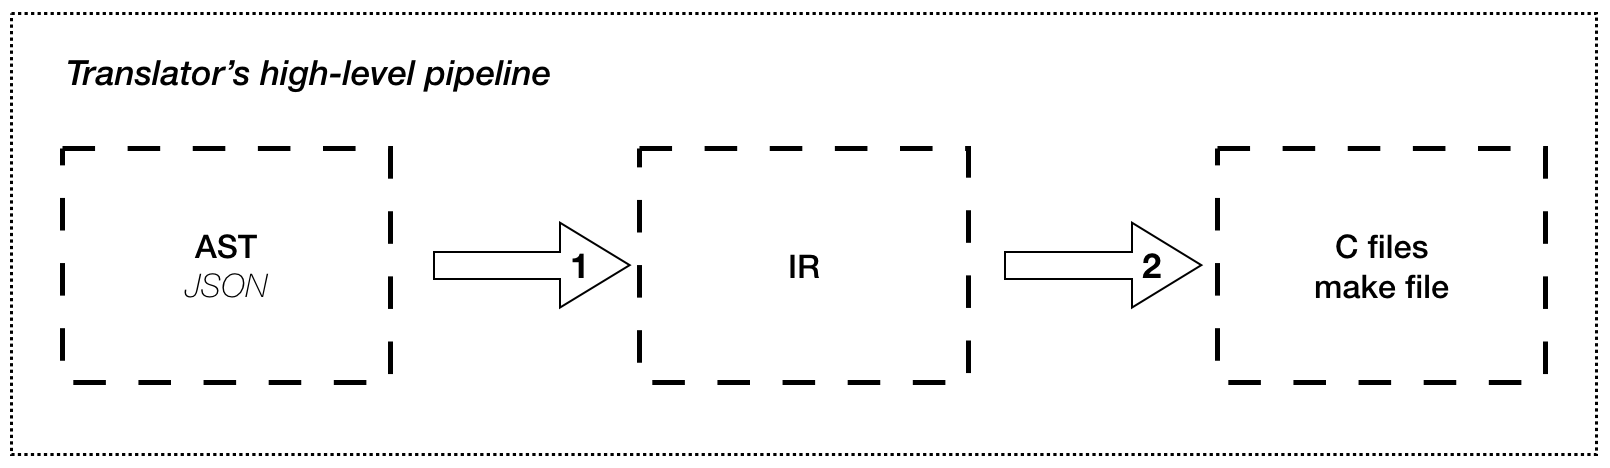
\includegraphics[width=\linewidth]{Translators_high_level_pipeline.png}
    \caption{Translator high-level pipeline}
    \label{fig:plan}
\end{figure}

\subsection{Proposed architecture}
The proposed solution is structured as follows: while parsing AST, a tree consisting of classes representing AST nodes -- semantic language entities, such as functions, variables and many more -- is built.
A separate class represents every entity, and every class implements the Constructible interface, which contains the construct() method, that returns a text string containing the corresponding code in C. If a class object refers to other objects (i.e., representation of function declaration which contains variable declarations), then inside construct() of the parent object construct() for all child objects is called recursively, and this is what happens to all the objects that are Constructible. In other words, the construct() method performs the traversal of the tree built while parsing AST, in an appropriate order.

Almost all Constructible classes have attributes, which store metadata needed to build a specific construction, and are defined during the object creation, inside a constructor. For example, a function will have such attributes as name, return type, function arguments (signature) and function body. All attributes should also implement Constructible to fit the proposed idea of recursive calls of construct().

To build expressions, certain patterns are used; these are the stubs of source code in C, that have fields to be replaced by certain attributes after they are constructed. For instance, the pattern for function declaration looks as follows:

\begin{lstlisting}[numbers=none]
    RET_TYPE  FUNC_NAME  ( SIGNATURE )  { BODY }
\end{lstlisting}
Here we can see four placeholders to be replaced by return type, function name, function argument list and function body respectively.

Interestingly, this approach is suitable for implementation of simple examples of code for many different programming languages, e.g., for Python, which is syntactically distant from C:

\begin{lstlisting}[language=Python, numbers=none ]
    def  FUNC_NAME  ( SIGNATURE )  ->  RET_TYPE: \n\t BODY
\end{lstlisting}


This example would only allow generating simple functions with a single line in a function body. Still, the mere possibility to describe different programming language constructs enforces the thought that the concept can be expanded to such a level that to enable code generation into one more language one will only need to create a file with patterns to describe it adequately.

% Данный пример подходит только для генерации простых функций с одной строкой в теле. Но сама возможность создания языковых конструкций различных языков заставляет задуматься о расширении генератора до уровня, когда для добавления нового языка потребуется только создать соответствующий файл шаблонов.

% \subsection{Issues in C}
% Undefined behaviour


\section{An approach implementation OOP in C}
The notion of OOP usually implies following at least three main principles: inheritance, polymorphism, and encapsulation.

\begin{itemize}
    \item \textbf{Inheritance} is an ability of objects of a particular type to inherit properties and methods of some other type for the further use.

    \item \textbf{Polymorphism} is a possibility for objects with the same interface and specification to have a different implementation which is possible, for example, when implementation of some parts of the class was changed in the course of inheritance.

    \item \textbf{Encapsulation} is a possibility to hide a class implementation and provide an interface for interacting with objects of this class.
\end{itemize}

These are precisely principles that are necessary to be implemented for a language to be considered object-oriented.

It is also worth noting that the OO approach has specific issues within. For instance, there exists a so-called diamond problem: while inheriting a class from two parents with identically named fields or methods, the overlapping happens, which becomes the reason why it is not defined which parent gave the class a given field or method. Since language creators have not yet decided on the solution, for now, we will not make this issue a center of attention.

Axel-Tobias Schreiner describes methods of implementation of the object-oriented paradigm in C in his book ``Object-oriented programming with \mbox{ANSI-C}''\cite{Schreiner2011}. 
Let us now consider a few ways of how ideas from this book are going to be used in the proposed solution.
%In this thesis, some ideas from this book are going to be used, as necessary. 

\subsubsection{Inheritance}
In C, inheritance can be implemented through aggregation of an instance of a parent class, Figure \ref{fig:C_inh_scheme}. Just like with ordinary class declaration, the class is defined using ``typedef struct'', the only difference is that with inheritance, the base class object is listed as one of the fields. The constructor of the derived class calls a constructor of a base class. From the user’s point of view, the work with a derived class is absolutely the same as with a class without inheritance.

\begin{figure}[h!]
    \centering
    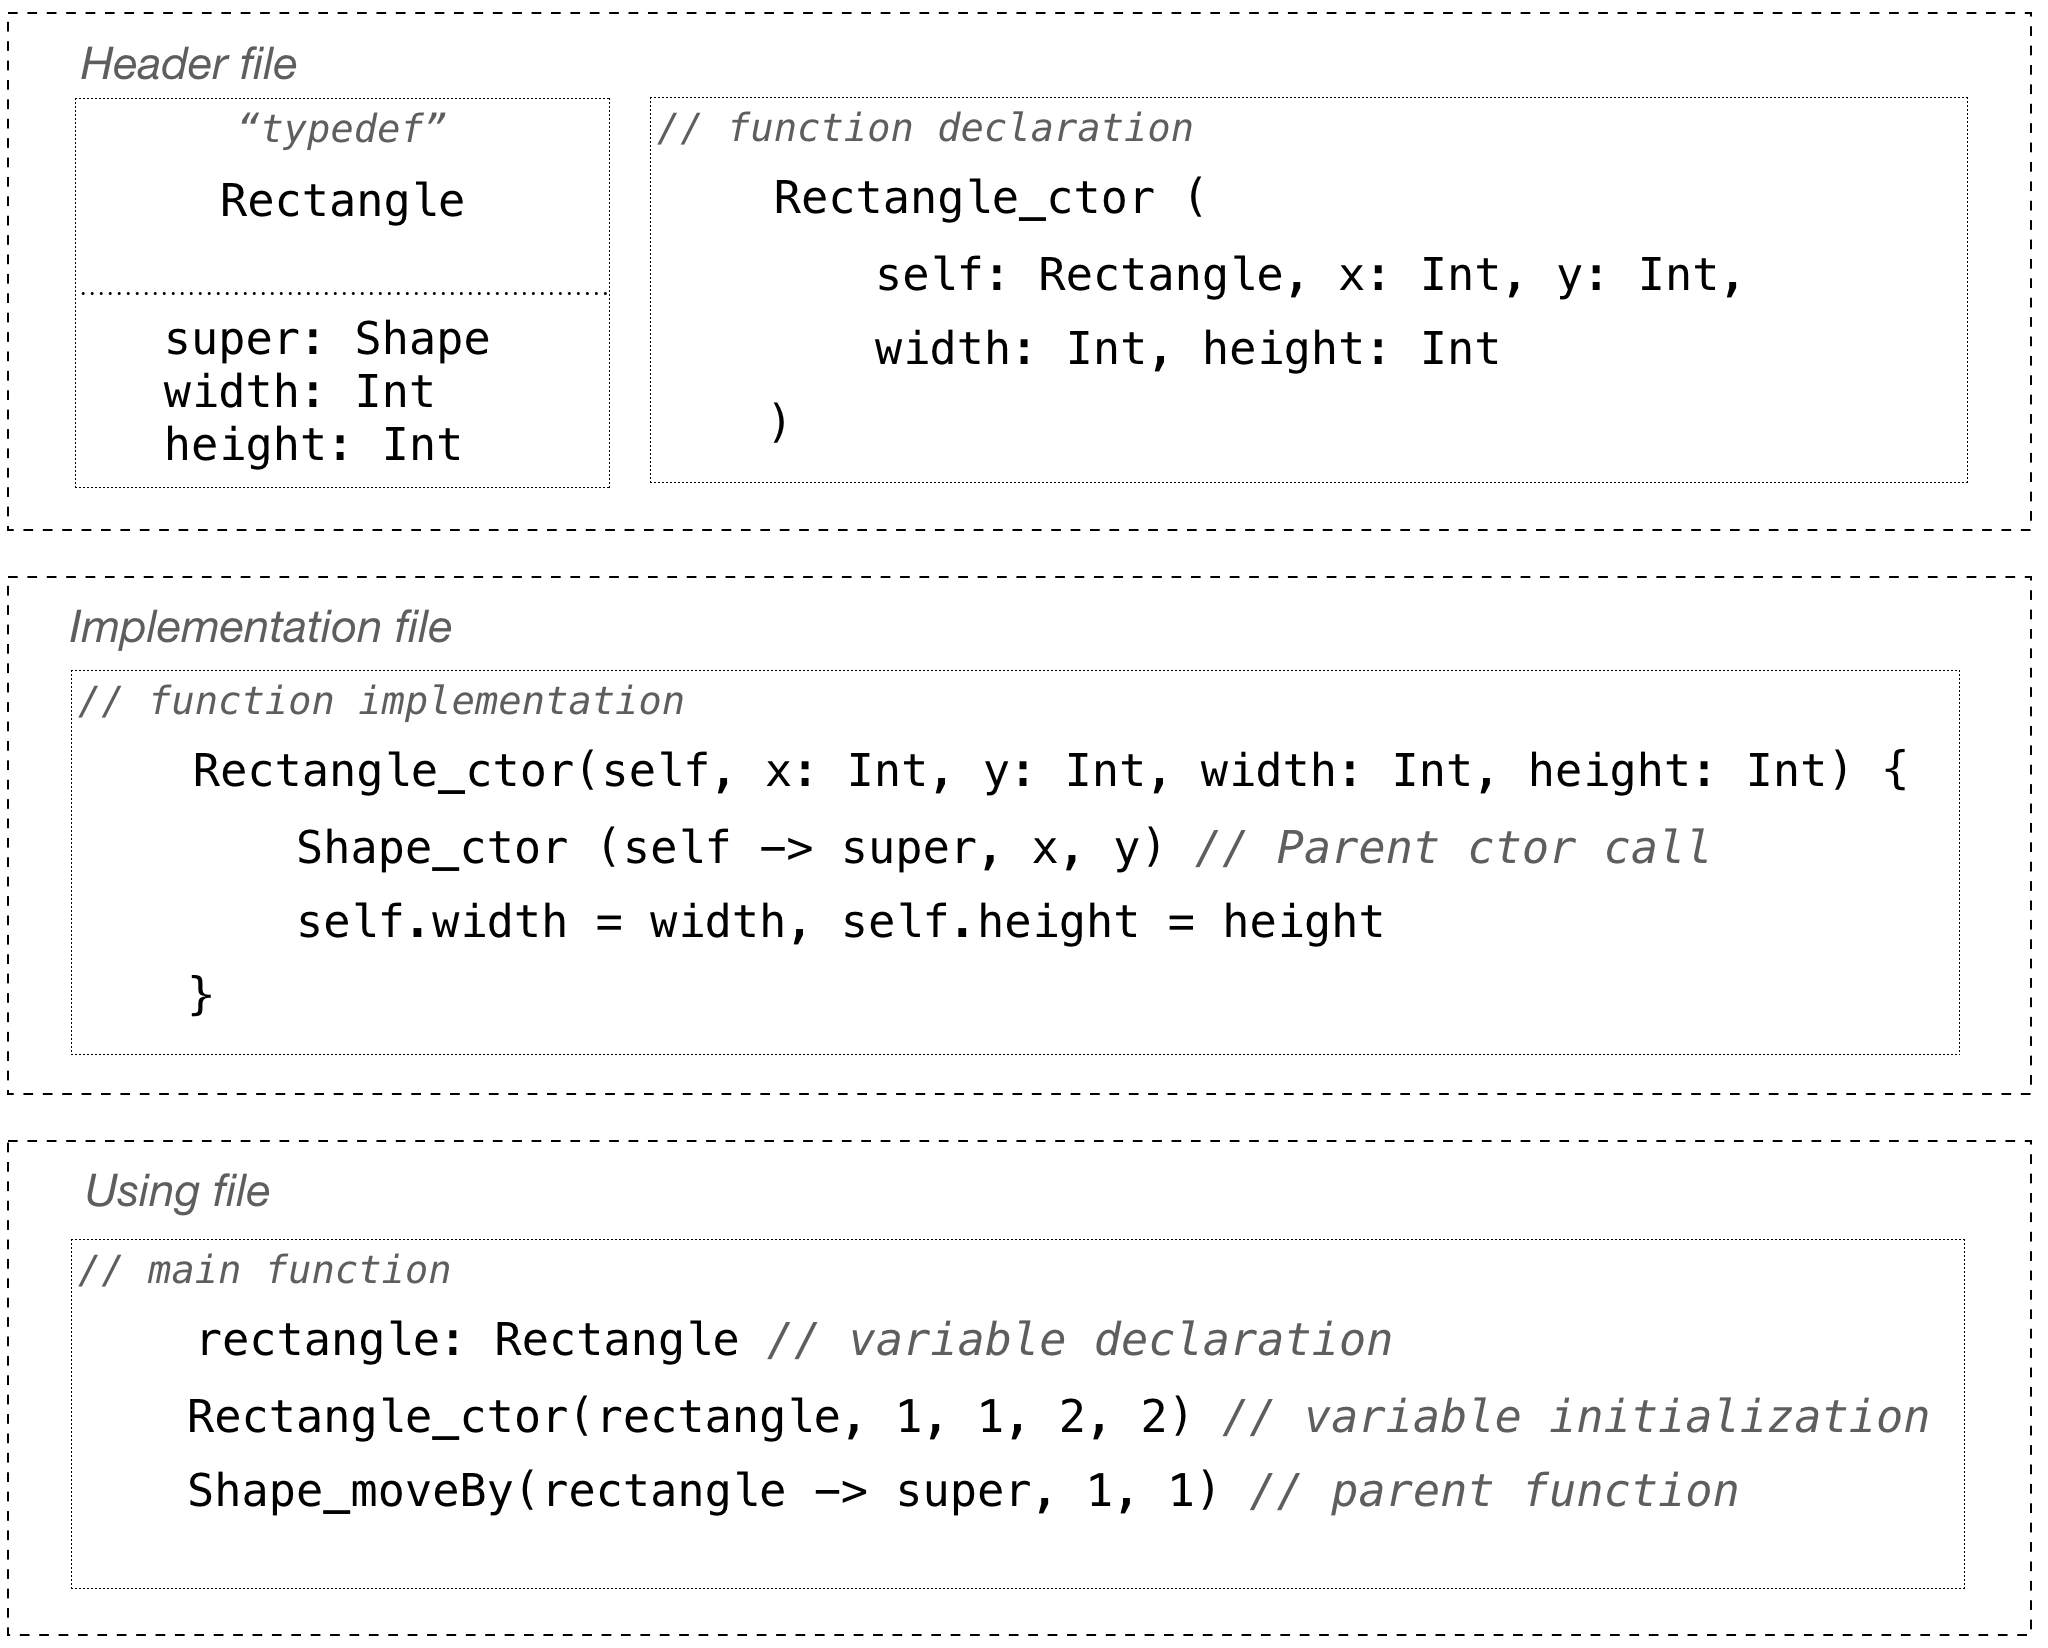
\includegraphics[width=\linewidth]{C_inh_scheme.png}
    \caption{Inheritance in C}
    \label{fig:C_inh_scheme}
\end{figure}

\subsubsection{Encapsulation}
In this thesis, encapsulation in the sense of access modifiers is not necessary to port object-oriented programs into C, as all the needed access checks are performed during generation of AST.

\subsubsection{Polymorphism}
Polymorphism implies the use of the common interface by similar classes, which is a much harder task than anything described above, as it cannot possibly be implemented without auxiliary constructs such as C++ virtual tables. 
Here, virtual tables are structures where pointers to ``virtual'' functions are declared. 
Consider the class as mentioned earlier Shape, with added functions area() and draw() that would calculate the shape area and draw the shape, respectively. 
Of course, it is not possible to calculate an area of an abstract shape or to draw an abstract shape. Thus these functions will be, in C++ terms, pure virtual, that is, required to be implemented by Shape descendants. On the Fig \ref{fig:C_UML} we can see the UML diagram of Shape along with Rectangle and Circle derived from it.

\begin{figure}[h!]
    \centering
    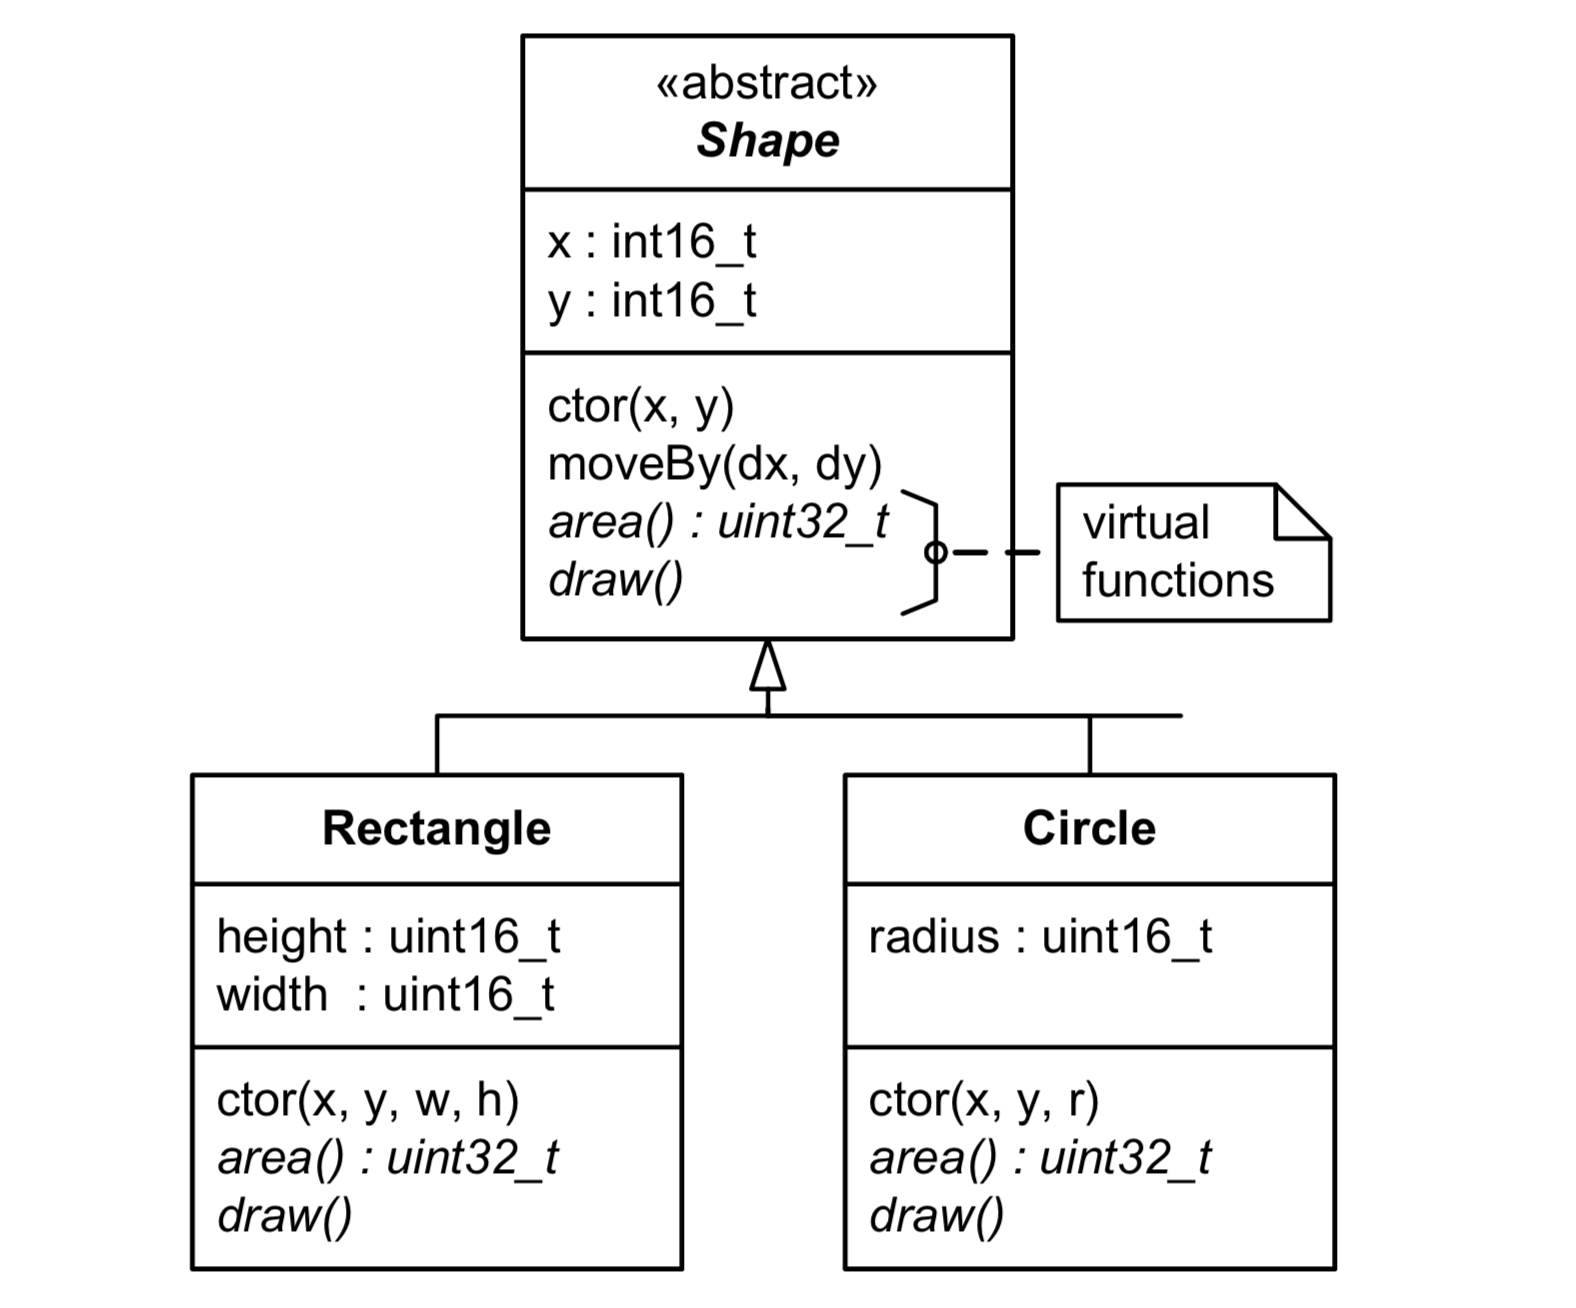
\includegraphics[width=\linewidth]{C_UML.png}
    \caption{Polymorphism in C, UML}
    \label{fig:C_UML}
\end{figure}

\subsection{Class declaration}
Consider the class Shape written in SLang:
\begin{lstlisting}[morekeywords={unit, end, is}, caption={Class declaration in Slang}, label={lst:Slang_class_decl}]
unit Shape 
    x: Int
    y: Int

    moveBy(dx: Int, dy: Int) is
        x += dx
        y += dy
    end moveBy
end
\end{lstlisting}

On the figure \ref{fig:C_class_decl_scheme} the declaration of the aforementioned class is schematically described. Declaration of the type and its methods is placed into the separate header file, and the type itself is declared using ``typedef struct''. In the associated source file the class methods are implemented. Methods use a pointer to a class object as the first argument to work with it. On the scheme, they are denoted as ``self''. Thus the object creation is creating a variable of the type of our class, and method call is performed by calling an associated function and passing the pointer to the object as the first parameter. The full Listing \ref{lst:C_class_decl} is available in the chapter \ref{chap:application}.

\begin{figure}[h!]
    \centering
    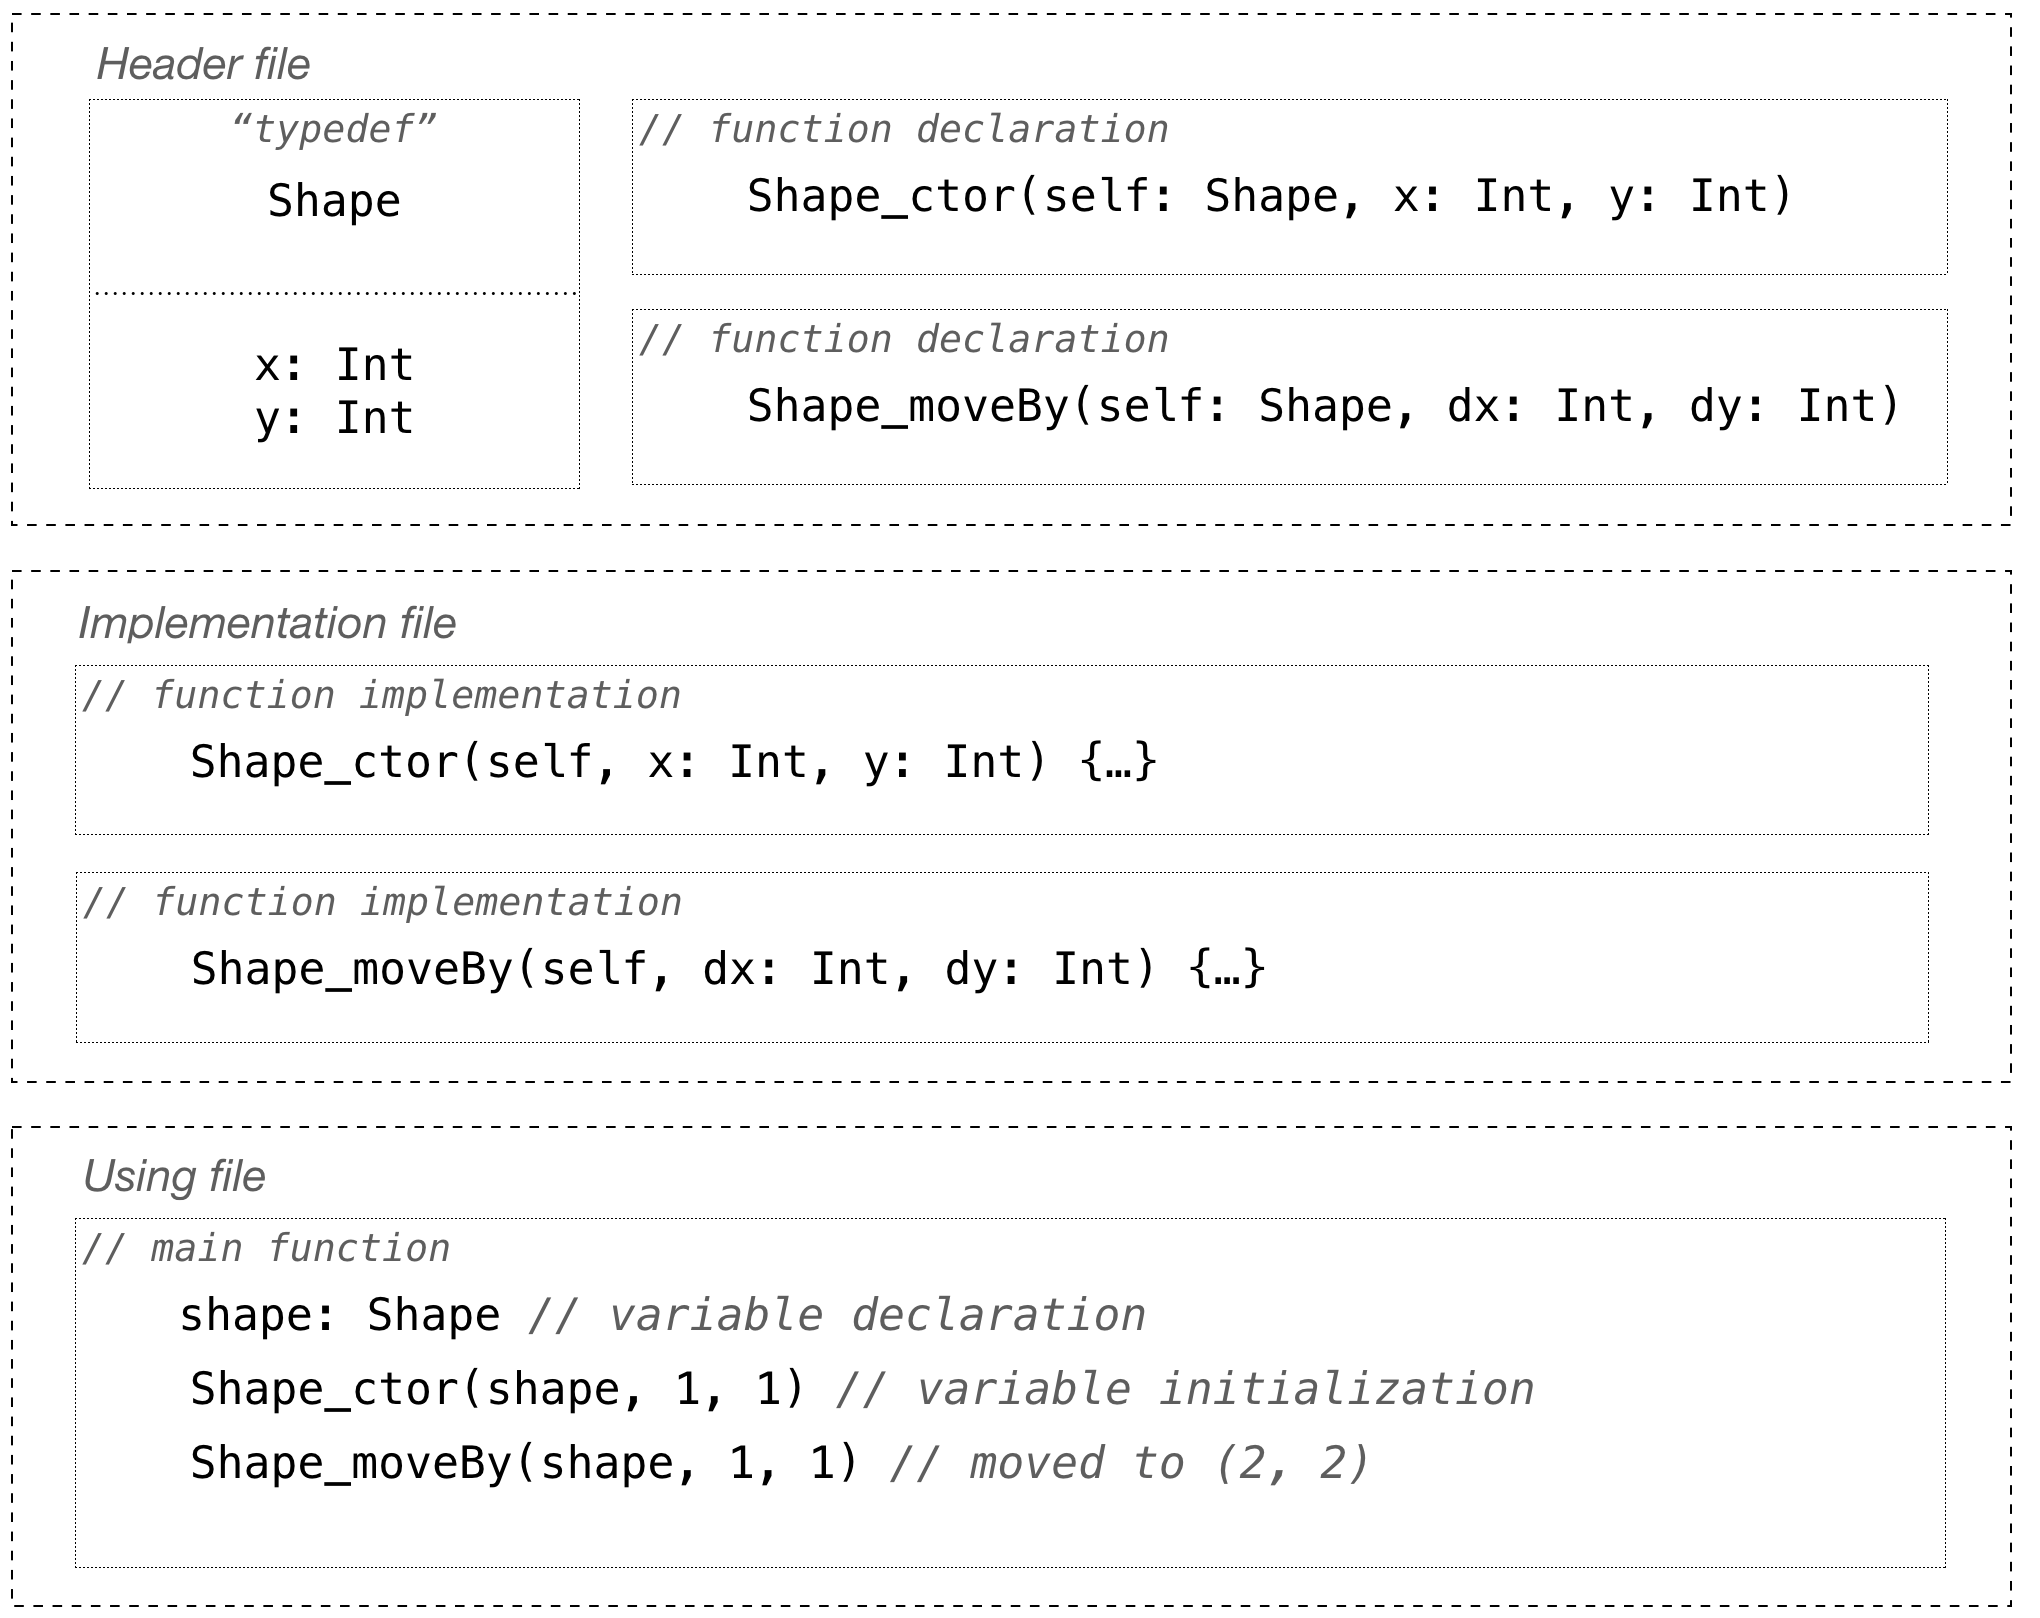
\includegraphics[width=\linewidth]{C_class_decl_scheme.png}
    \caption{Class declaration in C}
    \label{fig:C_class_decl_scheme}
\end{figure}


\subsection{Virtual table and Virtual pointer}
To implement the mechanism of virtual functions, we need a virtual table (vtbl) and a virtual pointer (vptr), which is going to be a part of a class. Virtual table as implemented in C is going to be a structure aggregating pointers to functions that are supposed to be virtual, as follows in Fig \ref{fig:ShapeVtblAndDecl} а), or Listing \ref{lst:Shapt_virt_table}.

Virtual Pointer is a pointer to the Virtual Table of the class. It must be defined for every instance of the class, which is to be done via making it one of the class fields. For example, the inner structure of the shape class can be seen on the Fig \ref{fig:ShapeVtblAndDecl} b) or in Listing \ref{lst:Shapt_virt_pointer}:

\begin{figure}[h!]
    \centering
    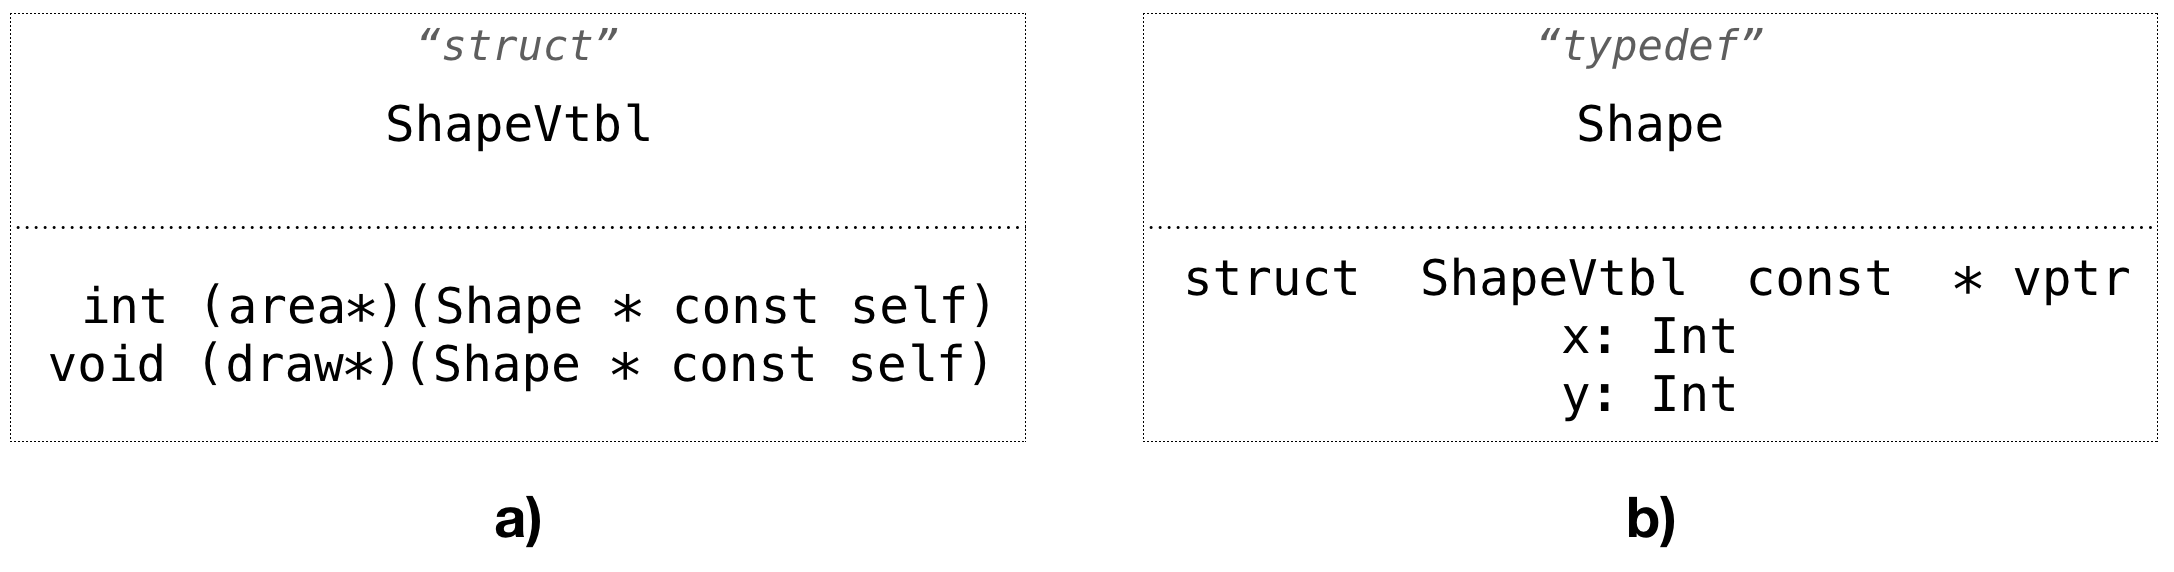
\includegraphics[width=\linewidth]{ShapeVtblAndDecl.png}
    \caption{ShapeVtbl struct declaration: a and Shape class declaration: b)}
    \label{fig:ShapeVtblAndDecl}
\end{figure}


\subsection{Setting the vptr in the Constructor}
For every instance of the class, its virtual pointer must be set to the corresponding virtual table, preferably on object creation, which implies that class’ constructor would be a perfect place to do that, Listing \ref{lst:Shape_vtbl_vptr}, Figure \ref{fig:Shape_vtbl_vptr_assignment}. 

\begin{figure}[h!]
    \centering
    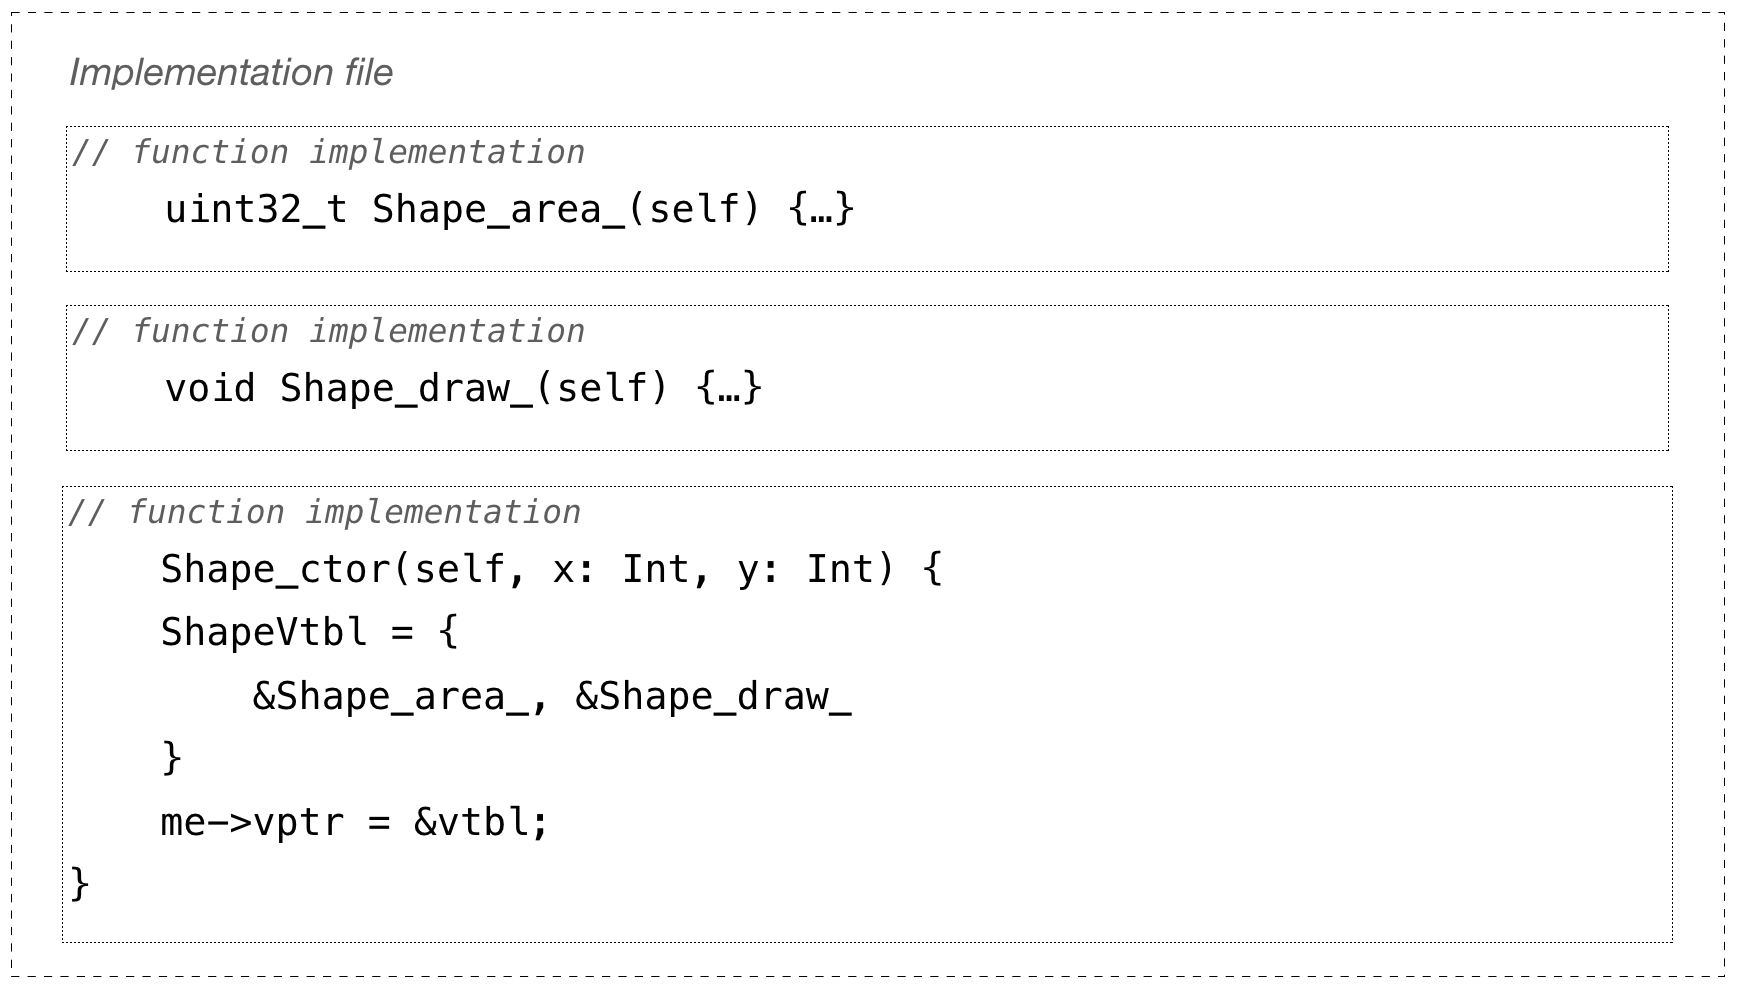
\includegraphics[width=\linewidth]{Shape_vtbl_vptr_assignment.png}
    \caption{Defining the virtual table and initializing the virtual pointer}
    \label{fig:Shape_vtbl_vptr_assignment}
\end{figure}

If a reasonable implementation of a virtual function cannot be provided in a class, which happens in case of abstract classes, implementations should ensure they interrupt the runtime (as they would not work in object-oriented languages in any case) with smart use of asserts, Listing \ref{lst:Pure_virt}.

\subsection{Inheriting the vtbl and Overriding the vptr in the Subclasses}
Due to the way inheritance is implemented, vptr is inherited automatically if present in the base class, by all subclasses at all levels, so for polymorphic classes, the principle of attribute inheritance works automatically.

Nevertheless, for every specififc subclass vptr needs to be reassigned to the respective vtbl, which also is to happen inside a constructor. For instance, consider the constructor of the Rectangle class, derived from Shape:

\begin{lstlisting}[caption={Overriding the vtbl and vptr in the subclass Rectangle}, label=lst:Overriding_vtbl_vptr]
/* Rectangle's class implementations of its virtual functions*/ 
static uint32_t Rectangle_area_( * const me);
static void Rectangle_draw_( * const me);
/* constructor */
void Rectangle_ctor(Rectangle * const me, int16_t x, int16_t y,
uint16_t width, uint16_t height)
{
    static struct ShapeVtbl const vtbl = { 
        /* vtbl of the Rectangle class */
        &Rectangle_area_,
        &Rectangle_draw_
    };
    Shape_ctor(&me->super, x, y); /*call the superclass' ctor*/
    me->super.vptr = &vtbl; /* override the vptr */
    me->width = width;
    me->height = height; 
}
\end{lstlisting} 

First of all, to initialize the me->super member, which is necessarily a subobject of the type of the superclass, the Shape constructor is invoked. There, the vptr is set to Shape’s vtbl. However, in the next statement it is reassigned to the Rectangle’s vtbl, so the vptr is overridden.

To fit into the vtbl, all implementations of virtual functions that are made for a subclass must precisely match signatures predefined earlier in the superclass. For example, the implementation Rectangle\_area\_() takes the pointer “me” of type Shape*, not Rectangle*, exactly for this reason, so in the actual implementation, an explicit downcast should be performed, as in Listing \ref{lst:Downcasting_me}:

\begin{lstlisting}[caption={Explicit downcasting of the “me” pointer}, label=lst:Downcasting_me]
static uint32_t Rectangle_area_(Shape * const me) {
    Rectangle * const me_ = (Rectangle *)me; /* explicit downcast */
    return (uint32_t)->width * (uint32_t)me_->height;
}
\end{lstlisting}

\subsection{Virtual Call}
With the following infrastructure of Virtual Tables and Virtual Pointers, the virtual call (late binding) can be implemented like in the example below:
\begin{lstlisting}[]
uint32_t Shape_area(Shape * const me) {
    return (*me->vptr->area)(me);
}
\end{lstlisting}

The virtual call works by first de-referencing the vtbl of the object to find the corresponding vtbl and only then calling the appropriate implementation from this vtbl via a pointer-to-function. The figure \ref{fig:virtual_call_mech} illustrates this process.

\begin{figure}[h!]
    \centering
    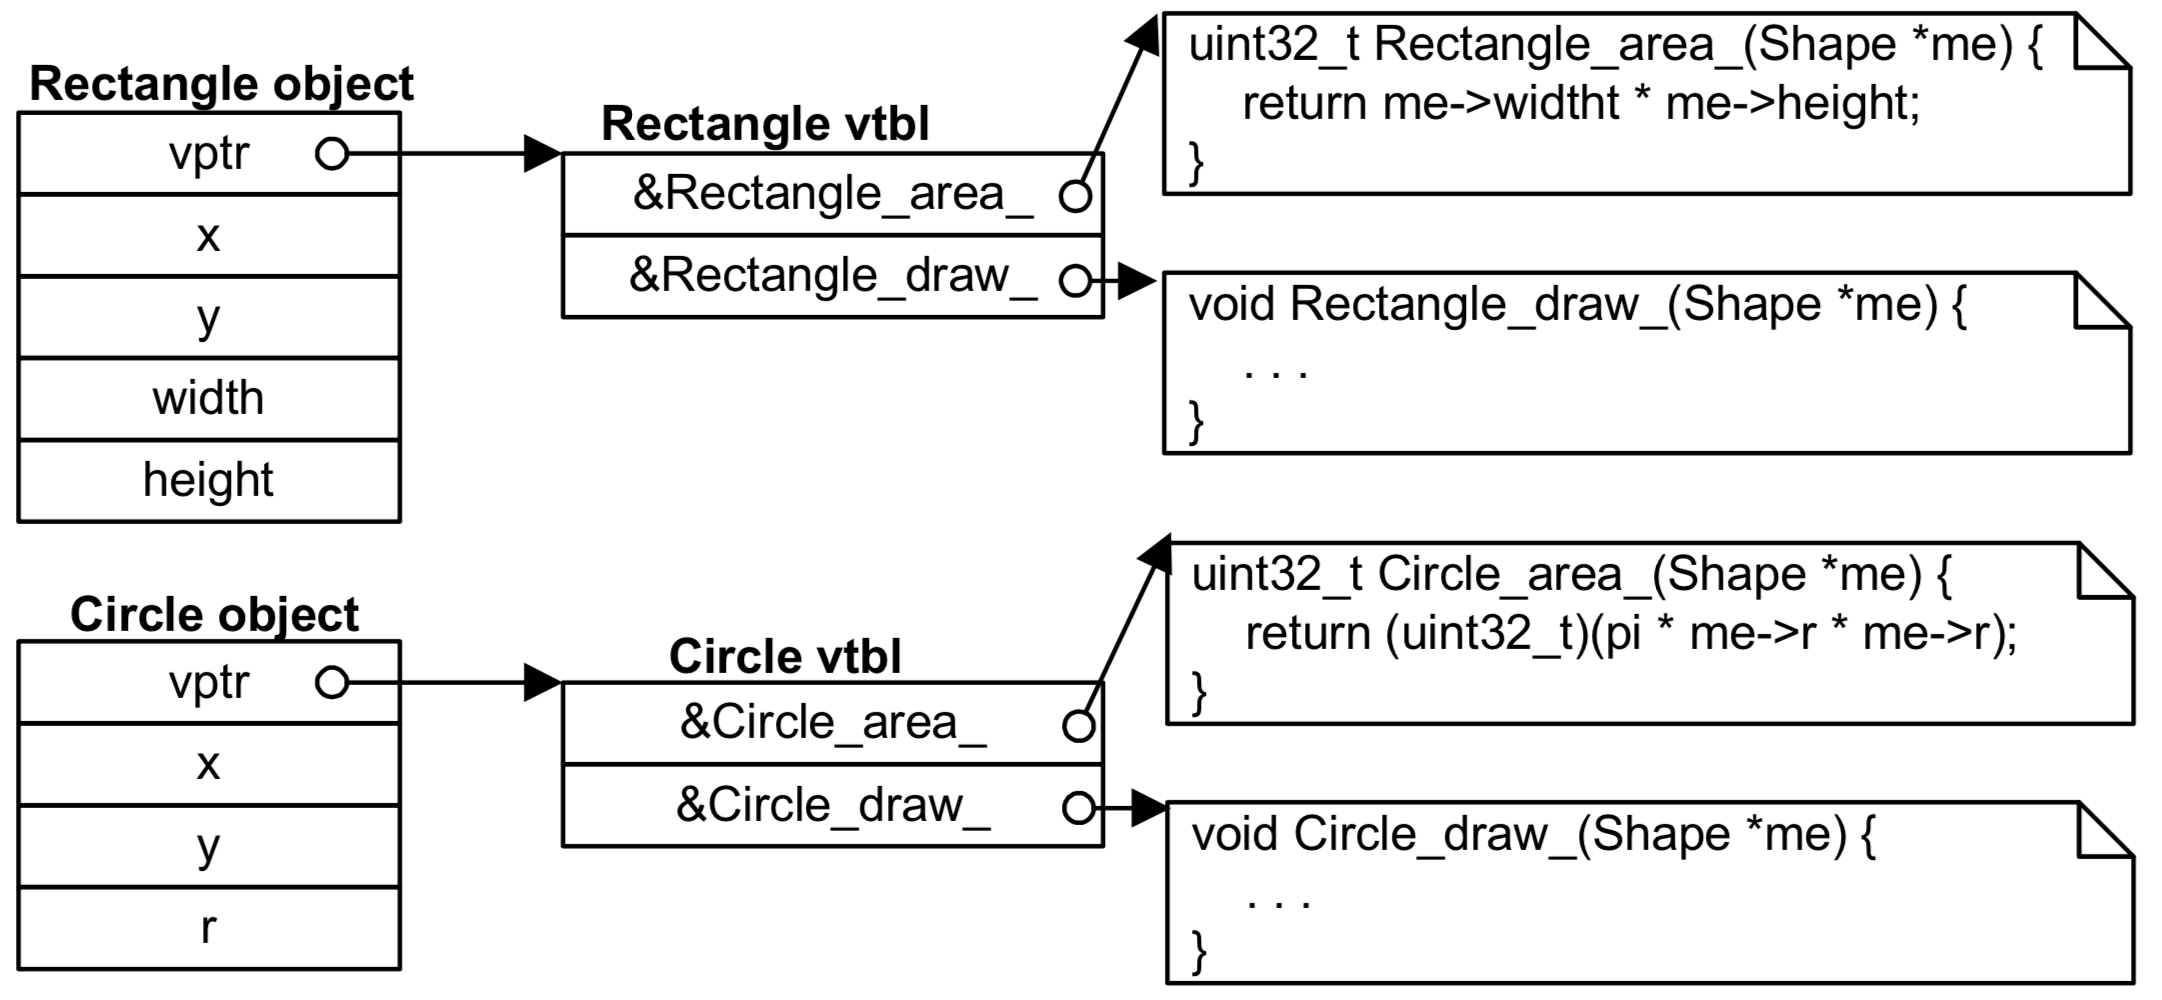
\includegraphics[width=\linewidth]{virtual_call_mech.png}
    \caption{Virtual call mechanism for Rectangles and Circles}
    \label{fig:virtual_call_mech}
\end{figure}

 
% Referencing other chapters \ref{chap:lr}, \ref{chap:met}, \ref{chap:impl}, \ref{chap:eval} and \ref{chap:conclusion}

\chapter{Implementation}
\label{chap:impl}


\section{Chosen programming language}
The proposed architecture of the translator implies large amounts of work with strings, and due to that, the Python programming language was chosen, as it is a language containing extensive functionality to work with text strings.
However, after the first prototype of the translator was implemented, it was found out that this language bears many difficulties in the task of implementation of the complete system. Thus it was decided to change the implementation language to Java, as it is one of the most widely used languages for multiple purposes.
After rewriting the prototype into Java, we realized that this language is all too bulky for the task --- for each new class, which were planned to be a vast multitude, it was necessary to create a separate file for the source code. 
With this issue in mind, finally the Kotlin programming language was chosen, due to it being the most suitable for the implementation: on the one hand, it is as powerful as Java, and on the other hand, as compact and expressive as Python.


\section{Prototype implementation details}
SLang is designed to be a multiparadigm programming language, so due to this fact it was decided to implement the system in a paradigm-by-paradigm fashion, starting with the simplest paradigms, then moving to more complex ones.
For a start, it was vital to implement basics of imperative programming: variable declaration and assignment, loops and branches.
After that, the next step was procedural programming --- function declaration, definition, and calls; the next one --- the introduction of OOP basics: simplistic classes, with fields and methods.
As stated in the previous chapter, there was no need to implement encapsulation, since it would unnecessarily complicate the situation, since most of the restrictions customarily forced by encapsulation are enforced over the course of analysis of the source code and AST construction. Instead, only inheritance and polymorphism were implemented. After that, it was decided to implement I/O and work with files as necessary programming elements in any language.

\section{Basic translator architecture}
All the architecture is designed in a way to implement the concept mentioned above of patterns: each pattern, which reflects one of the language constructs, is mapped to a class that implements the Constructable interface, which contains the construct() method, designed to use a pattern to substitute parameters inside it.
The language constructs, following the target language grammar, are nested, which is represented in the translator as the recursive aggregation of Constructable classes. The structure of this aggregation tree is a total copy of an input program AST.
The entry point of a program to be translated is represented with the EntryPoint class, which then contains all the other elements of the program.
The source code retrieval process launch is done via calling the construct() method, which performs a recursive walk across the aggregated instances, calling construct() inside every single one. This way, the process of the translation into the target source code is similar to AST walk, with the only difference that in this case, for every tree node the target language source code snippet is generated.

The translator source code files are split into several directories:
\begin{itemize}
    \item \textbf{language\_primitives} --- The source code files which contain basic language constructs, as well as the basic translator logic.
    \item \textbf{additional} --- Necessary utilities, used over the course of the work with translator.
    \item \textbf{mains} --- A directory for entry point files -- in each of them, there is a certain program in C, in the translator internal representation, ready for translation.
    \item \textbf{json\_patterns} --- Contains JSON-encoded patterns for different target programming languages. By now, patterns for C and JS are present.
\end{itemize}

\begin{figure}[h!]
    \centering
    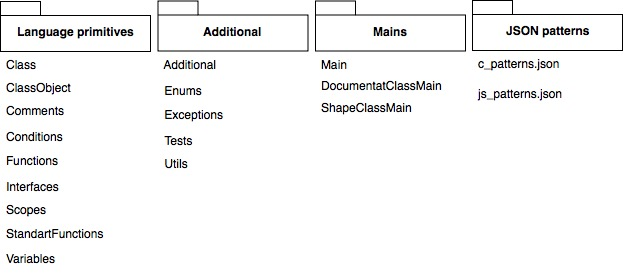
\includegraphics[width=\linewidth]{Thesis_UML.jpg}
    \caption{Project structure}
    \label{fig:Project_structure}
\end{figure}


\section{Implementation details}

\subsection{Patterns file}
The patterns file is a JSON file, which is divided into several parts:
\begin{itemize}
    \item The header part, which contains the pattern file version and a target language for the code generation. Both fields are not used for now and are rather done for the sake of future extension since the architecture allows code generation for multiple programming languages, as well as several versions of pattern files are possible.
    \item The patterns that represent the syntax of a target language.
    \item The list of standard libraries and functions contained in them: \textbf{dependencies} --- necessary for the sake of use of standard functions of a target language to project the functionality from SLang. Examples include console I/O.
    \item The list of standard functions of a target language: {standard\_functions} --- unlike the previous part, here is a place to describe every standard library function in a target language, if any. For instance, for the C programming language, we included functions printf() and scanf() as examples.
    \item A list of standard types in a target language: \textbf{standard\_types} --- to project SLang types onto the target language.
\end{itemize}

Moreover, there is a possibility of adding new sections to the format, depending on a target language and a patterns file version, depending on the evolving translator architecture. The way a pattern file looks can be seen in \ref{lst:Json_patterns}.

Such a way of pattern organization is suitable for source code generation into such languages as C, C++, Java, Kotlin, C\#, and Swift.
Moreover, over the course of translator architecture and pattern file format rework, it is theoretically possible to generate basic language constructs of languages similar to Python, JavaScript, and some others.
As an experiment, it was attempted to write patterns for JS, as well as writing a simplistic HelloWorld in it.
Results can be seen in the ``DocumentClassMain.kt'' file in ``mains'' package of the translator project directory, while a file with patterns is shown in Appendix \ref{lst:Json_JS_patterns}, as well as in the project directory.


\subsubsection{A technicality}
Since patterns are stored in a file, and disk I/O is time costly, it was decided to cache all the pattern data on the first file access, which is implemented inside the ``PatternsLoader'' class in ``Utils.kt'' in the ``additional'' package.

\subsection{Class Object}
In this implementation, in an inheritance model, for each class, virtual tables are created, along with a pointer to a parent object. Thus a natural question arises, namely what the parent of the class which is highest along the hierarchy is.
There can be two actual variants: either NULL or some class Object, which is the base class for all the created classes like it is done in Java. In SLang, the second approach was chosen, as it allows creating methods necessary for all objects, such as toString(), hashCode() and similar. Also, such approach allows not thinking about how to process the NULL parent.

\subsection{Kotlin implementation moments}
In this implementation, each language construct of a target language is mapped onto some class. 
Thanks to this architecture and Kotlin language features, the internal representation for many language constructs is implementing through inheriting from the Patternable abstract class, where the patternTyped field is overridden. The field has ``PATTERN\_TYPES'' type, which is an enum class, where each member is representative of a specific pattern.

Overall, enum classes are used quite widely in the translator. As of the time of writing, there are four of them:
\begin{itemize}
    \item \textbf{PATTERN\_TYPES} explained above, mapped ontpo patterns for every language construct;
    \item \textbf{EXPR\_TYPES}, used to denote an expression in a pattern, such as ``BODY'', ``VAR\_NAME'', ``LIB'' and similar;
    \item \textbf{STD\_TYPES} --- the list of standard types, commonly used in most of languages, such as ``INT'', ``REAL'', ``VOID'';
    \item \textbf{STD\_FUNCTIONS} --- the list of standard function concepts, existing in most of languages, such as console input and output.
\end{itemize}

\subsection{Makefile generation}
The makefile generation is done with the same technology, using patterns. The general makefile structure is shown in Appendix \ref{lst:C_make}.
Over the course of intermediate representation recompilation, the names of all source code files are put into a specially designed list, which is put into the SOURCES variable of the makefile, while the name of the file containing the entry point is put into EXECUTABLE. 
The compiler name and version is put into the CC variable, and then, necessary launch flags are optionally assigned to CFLAGS and LDFLAGS.

\section{The current implementation stats}
As of the time of writing, the following language constructs generation is implemented:
\begin{itemize}
    \item Classes, with fields, methods, and inheritance;
    \item The Object base class, as a base for all other classes;
    \item Line comments;
    \item Branching operators (if-else);
    \item Function declarations and calls;
    \item Variables: declaration, definition and usage;
    \item Imports from standard library depending on standard function calls;
    \item Standard basic I/O functionality;
\end{itemize}


\section{The structure of a resulting C project}
The structure is going as follows:
\begin{itemize}
    \item  Classes are put into source code files and headers.
    \item  Since for all classes Object is the base one, it will also be present in project files.
    \item  The makefile is generated to ensure a proper project build.
\end{itemize}


\section{The translator testing strategy}
The translator output is a sequence of strings. Thus, testing was performed as a comparison of the output to the reference strings. For each language construct, a test case was created, as a reference string for comparison. Since now there is no task of output beautification, while formatting is often changed over the course of translator implementation, it was decided to implement functionality for removal of redundant symbols from strings. This way, unit tests for the translator were implemented.
\chapter{Evaluation and Discussion}
\label{chap:eval}

\section{Immediate future work}
Potentially, the translator could be expanded with the following features:
\begin{itemize}
    \item Functional programming support;
    \item Contracts support;
    \item Full OOP support;
    \item Lambda functions support;
    \item Multiline comments support;
    \item Also, it is necessary to implement the AST parser for the translator, which would build the internal representation of a program according to its AST, to facilitate optimizations. Since the architecture is built with this future feature in mind, it should be relatively easy to implement the parser and merge it into the translator;
    \item An extensive CLI for the translator, with command line arguments;
    \item Nested functions;
\end{itemize}


\section{Possible problems}
In this kind of translator software, the problem of standard typing occupies a special place. The point is, supposedly similar standard types of different programming languages can differ in structure, logic, or size.
For example, integer types can be 8 bit, 32 bit, or, say, arbitrarily long. They can also have different behavior upon overflow (either overflowing or panicking) or different bitwise structure. Surely this makes for different integers.
An even brighter example is a string. A string can be just a char array or an object; it can contain ASCII chars, Unicode chars, or valid UTF8 (multibyte chars); it can be zero-terminated, zero-prohibitive or zero-permissive, and also mutable or immutable. The differences can be so vast that there is often a need to create a custom string structure in a target language to represent strings from the source language.
More globally, this can also refer to type mutability, or to questions whether a given instance is allocated on stack or in a heap, whether a given type is passed by value or by reference, and whether an object can be used only once or infinitely. Another interesting question is the average complexity of operations on resulting types which had also better be preserved. All these issues are what make the task of mapping type systems of different programming languages not entirely straightforward.
The aforementioned pattern system allows changing the mapped target language standard types quickly, which will help significantly to achieve full type compatibility.

\section{Proposed improvements and additions}
\begin{itemize}
    \item Over the course of translator implementation, there was an idea to adjust the translator architecture for C as the main target language. This kind of architecture would allow for more subtle optimizations for the target language, but also would restrict the adjustment to other languages while at the same time drastically increasing the complexity of the solution.
    \item Code generation into Python. The most special syntactic feature of the language is denoting the scopes with indentation. Due to a recursive way of target source code construction, it is possible to add indents according to recursion depth. This way, it is possible both to generate valid Python code and beautify code in other languages.
    \item For now, the translator makes no distinction between notions of expression and statement, which may negatively affect the translation. For example, now it is not yet possible to facilitate nested function calls. In the future, the addition of the difference between notions is necessary.
\end{itemize}
\chapter{Conclusion}
\label{chap:conclusion}

Over the course of the work on this thesis, a translator from SLang AST to C source code, which generated code based on fundamental programming paradigms, such as imperative, procedural and object-oriented programming, was implemented.
In the future, it is planned to introduce such paradigms as contract programming, functional programming, and many others, of those which are supported in SLang, until all features of this language are covered.

The resulting translator is quite perspective due to architecture allowing easy addition of new target languages.

The translator was tested on code snippets prepared in advance, having shown that semantic equivalence between the source and the target is respected, with some amount of assumptions.
\chapter{Application}
\label{chap:application}

\begin{lstlisting}[caption={Class declaration in C}, label={lst:C_class_decl}]
/* ---------------- Shape.h ---------------- */

/* Shape's attributes... */ 
typedef struct {
    int16_t x; /* x-coordinate of Shape's position */
    int16_t y; /* y-coordinate of Shape's position */ 
} Shape;

/* Shape's operations (Shape's interface)... */
void Shape_ctor(Shape * const me, int16_t x, int16_t y); 
void Shape_moveBy(Shape * const me, int16_t dx, int16_t dy);

/* ---------------- Shape.c ---------------- */

/* constructor */
void Shape_ctor(Shape * const me, int16_t x, int16_t y) {
    me->x = x;
    me->y = y; 
}
/* move-by operation */
void Shape_moveBy(Shape * const me, int16_t dx, int16_t dy) {
    me->x += dx;
    me->y += dy; 
}

/* Creating objects */ 
int main() {
    Shape s1, s2; /* multiple instances of Shape */
    Shape_ctor(&s1, 0, 1);
    Shape_ctor(&s2, -1, 2); 
    Shape_moveBy(&s1, 2, -4);
}
\end{lstlisting}

\begin{lstlisting}[caption={Inheritance in C}, label=lst:C_inheritance]
#include "Shape.h"
/* ---------------- Rectangle.h ---------------- */

typedef struct {
    Shape super; /* <== inherits Shape */ 
    /* attributes added by this subclass... */ 
    uint16_t width;
    uint16_t height;
} Rectangle;

/* constructor */
void Rectangle_ctor(Rectangle * const me, 
                    int16_t x, int16_t y, 
                    uint16_t width, uint16_t height);

/* ---------------- Rectangle.c ---------------- */
void Rectangle_ctor(Rectangle * const me, int16_t x, int16_t y,
uint16_t width, uint16_t height) 
{
    /* first call superclass ctor */
    Shape_ctor(&me->super, x, y);

    /* next, you initialize the attributes added by this subclass... */ 
    me->width = width;
    me->height = height;
}

/* Creating objects */ 
int main() {
    Rectangle r1, r2;
    /* instantiate rectangles... */ 
    Rectangle_ctor(&r1, 0, 2, 10, 15); 
    Rectangle_ctor(&r2, -1, 3, 5, 8);
    /* re-use inherited function from the superclass Shape... */ 
    Shape_moveBy((Shape *)&r1, -2, 3);
    Shape_moveBy(&r2->super, 2, -1);
}
\end{lstlisting}


\begin{lstlisting}[caption={Shape virtual table}, label={lst:Shapt_virt_table}]
struct ShapeVtbl {
    uint32_t ( area* )(Shape * const me); 
    void ( draw* )(Shape * const me);
};
\end{lstlisting}


\begin{lstlisting}[caption={Adding virtual pointer to Shape class}, label={lst:Shapt_virt_pointer}]
struct ShapeVtbl; /* forward declaration */ 
typedef struct {
    struct ShapeVtbl const *vptr; /* <= Shape's vptr */
    int16_t x;
    int16_t y;
} Shape;
\end{lstlisting}


\begin{lstlisting}[caption={Defining the virtual table and initializing the virtual pointer}, label={lst:Shape_vtbl_vptr}]
/* Shape class implementation of its virtual functions... */ 
static uint32_t Shape_area_(Shape * const me);
static void Shape_draw_(Shape * const me);
/* constructor */
void Shape_ctor(Shape * const me, int16_t x, int16_t y) {
    static struct ShapeVtbl const vtbl = { 
        &Shape_area_,
        &Shape_draw_
    };
    me->vptr = &vtbl; /* "hook" the vptr to the vtbl */

    me->x = x;
    me->y = y; 
}
\end{lstlisting}


\begin{lstlisting}[caption={Defining purely virtual functions}, label={lst:Pure_virt}]
/* Shape class implementations of its virtual functions... */ 
static uint32_t Shape_area_(Shape * const me) {
    ASSERT(0); /* purely-virtual function should never be called */
    return 0; /* to avoid compiler warnings */ 
}
    
static void Shape_draw_(Shape * const me) {
    ASSERT(0); /* purely-virtual function should never be called */
}
\end{lstlisting}

\lstset{
  language=json,
  breaklines=true,
  frame=L,
  basicstyle=\footnotesize\ttfamily,
  morekeywords={version, language, patterns, dependencies, standard_types, standard_functions}
}

\begin{lstlisting}[caption={Patterns JSON file for C language}, label={lst:Json_patterns}]
{
  "version": 0.1,
  "language": "C",
  "patterns": {
    "STR_VAR": {
      "pattern": "\""
    },
    "CHAR_VAR": {
      "pattern": "'"
    },
    "LOOP": {
      "pattern": "for(INITIAL_STATE, WHILE_CONDITION, STEP_EXPR){BODY}"
    },
    "IF_CONDITION": {
      "pattern": "if(CONDITION){\nBODY\n}"
    },
    "ELSE_CONDITION": {
      "pattern": "else{\nBODY\n}"
    },
    "ELIF_CONDITION": {
      "pattern": "else if(CONDITION){BODY}"
    },
    "TERNARY": {
      "pattern": "CONDITION?TRUE:FALSE;"
    },
    "FUNC_DECL": {
      "signature_delimiter": ",",
      "pattern": "\nRET_TYPE FUNC_NAME(SIGNATURE){\nBODY\n}"
    },
    "ENTRY_POINT": {
      "signature_delimiter": ",",
      "pattern": "\nRET_TYPE FUNC_NAME(SIGNATURE){\nBODY\n}"
    },
    "FUNC_CALL": {
      "signature_delimiter": ",",
      "pattern": "FUNC_NAME(PARAMS);"
    },
    "SIG_PARAM": {
      "pattern": "RET_TYPE VAR_NAME"
    },
    "SIG_PARAM_POINTER": {
      "pattern": "RET_TYPE *VAR_NAME"
    },
    "SIG_PARAM_CONST_POINTER": {
      "pattern": "RET_TYPE *const VAR_NAME"
    },
    "VAR_DECL": {
      "pattern": "RET_TYPE VAR_NAME;"
    },
    "VAR_DECL_POINTER": {
      "pattern": "RET_TYPE *VAR_NAME;"
    },
    "VAR_ASSIGNMENT": {
      "pattern": "VAR_NAME = VALUE;"
    },
    "EMPTY_OPERATOR": {
      "operator": ";"
    },
    "DEPENDENCY": {
      "pattern": "#include <LIB>"
    },
    "VAL_STR": {
      "pattern": "\"VALUE\""
    },
    "VAL_INT": {
      "pattern": "VALUE"
    },
    "HEADER_FILE": {
      "pattern": "#ifndef TYPE_ALIAS_H\n#define TYPE_ALIAS_H\ntypedef struct {\nMEMBER_DECLARATIONS\n} TYPE_ALIAS; FUNCTION_PROT_DECLARATIONS\n#endif"
    },
    "CLASS_DECL": {
      "pattern": "#include \"TYPE_ALIAS.h\"\nFUNCTION_DECLARATIONS"
    },
    "FUNC_PROTOTYPE": {
      "signature_delimiter": ",",
      "pattern": "\nRET_TYPE FUNC_NAME(SIGNATURE);"
    },
    "FUNC_RETURN": {
      "pattern": "return VAR_NAME;"
    },
    "SYMBOLIC_SEQ": {
      "pattern": "VALUE"
    },
    "ONE_STRING_COMMENT": {
      "pattern": "// VALUE"
    }
  },
  "dependencies": {
    "stdio.h": ["printf", "scanf"],
    "sthlib.h": ["sth"]
  },
  "standard_types": {
    "STRING": "char*",
    "INT": "int",
    "REAL": "float",
    "CHAR": "char",
    "VOID": "void"
  },
  "standard_functions": {
    "console_out": {
      "name": "printf",
      "str": "%s",
      "int": "%d"
    },
    "console_in": {
      "name": "scanf",
      "str": "%s",
      "int": "%d"
    }
  }
}
\end{lstlisting}

\begin{lstlisting}[caption={Patterns JSON file for JavaScript language}, label={lst:Json_JS_patterns}]
{
  "version": 0.1,
  "language": "JavaScipt",
  "patterns": {
    "STR_VAR": {
      "pattern": "\""
    },
    "CHAR_VAR": {
      "pattern": "'"
    },
    "LOOP": {
      "pattern": "for(INITIAL_STATE, WHILE_CONDITION, STEP_EXPR){BODY}"
    },
    "IF_CONDITION": {
      "pattern": "if(CONDITION){\nBODY\n}"
    },
    "ELSE_CONDITION": {
      "pattern": "else{\nBODY\n}"
    },
    "ELIF_CONDITION": {
      "pattern": "else if(CONDITION){BODY}"
    },
    "TERNARY": {
      "pattern": "CONDITION?TRUE:FALSE;"
    },
    "FUNC_DECL": {
      "signature_delimiter": ",",
      "pattern": "function FUNC_NAME(SIGNATURE){BODY}"
    },
    "ENTRY_POINT": {
      "signature_delimiter": ",",
      "pattern": "BODY"
    },
    "FUNC_CALL": {
      "signature_delimiter": ",",
      "pattern": "FUNC_NAME(PARAMS)"
    },
    "SIG_PARAM": {
      "pattern": "VAR_NAME"
    },
    "SIG_PARAM_POINTER": {
      "pattern": "VAR_NAME"
    },
    "SIG_PARAM_CONST_POINTER": {
      "pattern": "VAR_NAME"
    },
    "VAR_DECL": {
      "pattern": "var VAR_NAME;"
    },
    "VAR_DECL_POINTER": {
      "pattern": "var VAR_NAME;"
    },
    "VAR_ASSIGNMENT": {
      "pattern": "VAR_NAME = VALUE;"
    },
    "EMPTY_OPERATOR": {
      "operator": ";"
    },
    "DEPENDENCY": {
      "pattern": "# LIB"
    },
    "VAL_STR": {
      "pattern": "\"VALUE\""
    },
    "VAL_INT": {
      "pattern": "VALUE"
    },
    "HEADER_FILE": {
      "pattern": "var TYPE_ALIAS = {MEMBER_DECLARATIONS\nFUNCTION_PROT_DECLARATIONS\n};"
    },
    "CLASS_DECL": {
      "pattern": "# TYPE_ALIAS | FUNCTION_DECLARATIONS"
    },
    "FUNC_PROTOTYPE": {
      "signature_delimiter": ",",
      "pattern": "# FUNC_NAME | SIGNATURE)"
    }
  },
  "dependencies": {},
  "standard_types": {
    "STRING": "",
    "INT": "",
    "REAL": "",
    "CHAR": "",
    "VOID": ""
  },
  "standard_functions": {
    "console_out": {
      "name": "console.log",
      "str": "%s",
      "int": "%d"
    },
    "console_in": {
      "name": "scanf",
      "str": "%s",
      "int": "%d"
    }
  }
}
\end{lstlisting}


\begin{lstlisting}[caption={C make file pattern}, label={lst:C_make}]
CC=g++
CFLAGS=-c -Wall
LDFLAGS=
SOURCES=LIST_OF_SOURCES
OBJECTS=$(SOURCES:.cpp=.o)
EXECUTABLE=EXECUTABLE_NAME

all: $(SOURCES) $(EXECUTABLE)
	
$(EXECUTABLE): $(OBJECTS) 
	$(CC) $(LDFLAGS) $(OBJECTS) -o $@

.cpp.o:
	$(CC) $(CFLAGS) $< -o $@
\end{lstlisting}
\lstset{
  language=C,
  basicstyle=\tiny,
  breaklines=true,
  numbers=none,
  frame=none,
  morekeywords={in, loop, end, unit, extend, override, Integer}
}
\begin{center}
\begin{tabular}{ | l | l | } \hline
SLang & Patterns \\ \hline
% CONDITION
\begin{lstlisting}
if CONDITION then
    // condition_true body
else
    // condition_false body
end
\end{lstlisting} & 
\begin{lstlisting}
if(CONDITION) {
    // condition_true body    
}
else {
    // condition_false body
}
\end{lstlisting} \\ \hline

% LOOP
\begin{lstlisting}
while ELEMENT in COLLECTION loop
    // loop body
end
\end{lstlisting} & 
\begin{lstlisting}
for(; ELEMENT != null; COLLECTION.next()){
    // loop body
    // where ELEMENT is sth like:
    // COLLECTION.getCurrentElement()
}
\end{lstlisting} \\ \hline

% CLASS
\begin{lstlisting}
unit Base
    x: Integer
    foo()
end
\end{lstlisting} & 
\begin{lstlisting}
typedef struct {
    int x;
} Base;
void Base_foo(Base* self){}
\end{lstlisting} \\ \hline

% INHERITANCE
\begin{lstlisting}
unit Derived extend Base, Base2
    y: Integer
    override foo()
end
\end{lstlisting} & 
\begin{lstlisting}
typedef struct {
    Base super;
    Base2 super2;
    int y;
} Derived;
Derived_foo(Derived* self){}
\end{lstlisting} \\ \hline

% NESTED FUNCTIONS
\begin{lstlisting}
foo(i: Integer) is
    boo(j: Integer, i: Integer) is 
        System.IO.print(i+j)
    end boo
    boo(1, i)
end foo
\end{lstlisting} & 
\begin{lstlisting}
void foo(int i) {
    void boo(int j, int i);
    boo(1, i);
}
void boo(int j, int i){
    printf("%d", i+j);
}
\end{lstlisting} \\ \hline
\end{tabular}
\end{center}

%% REFERENCES

\bibliography{my_thesis} 
\bibliographystyle{ieeetr}
% \appendix
\chapter{Extra Stuff}
\blindtext

\chapter{Even More Extra Stuff}
\blindtext
\end{document}

